% -*- Mode:TeX -*-

%% IMPORTANT: The official thesis specifications are available at:
%%            http://libraries.mit.edu/archives/thesis-specs/
%%
%%            Please verify your thesis' formatting and copyright
%%            assignment before submission.  If you notice any
%%            discrepancies between these templates and the 
%%            MIT Libraries' specs, please let us know
%%            by e-mailing thesis@mit.edu

%% The documentclass options along with the pagestyle can be used to generate
%% a technical report, a draft copy, or a regular thesis.  You may need to
%% re-specify the pagestyle after you \include  cover.tex.  For more
%% information, see the first few lines of mitthesis.cls. 

%\documentclass[12pt,vi,twoside]{mitthesis}
%%
%%  If you want your thesis copyright to you instead of MIT, use the
%%  ``vi'' option, as above.
%%
%\documentclass[12pt,twoside,leftblank]{mitthesis}
%%
%% If you want blank pages before new chapters to be labelled ``This
%% Page Intentionally Left Blank'', use the ``leftblank'' option, as
%% above. 

\documentclass[12pt,twoside]{mitthesis}
\usepackage{lgrind}
%% These have been added at the request of the MIT Libraries, because
%% some PDF conversions mess up the ligatures.  -LB, 1/22/2014
\usepackage{cmap}
\usepackage[T1]{fontenc}
\pagestyle{plain}

\hyphenation{block-chain}
\hyphenation{Block-chain}
\usepackage{rotating}
\usepackage{pdflscape}
\usepackage{subcaption}
\usepackage{tikz}
\usetikzlibrary{arrows}
\usepackage{amsmath}
%\usepackage[]{algorithm2e}
\usepackage{todonotes}
\presetkeys{todonotes}{inline}{}
\usepackage{algorithm}
\usepackage[noend]{algpseudocode}
\usepackage{multirow}
\usepackage{graphicx}
\graphicspath{{figures/}}
\usepackage{xcolor}
\definecolor{azure}{rgb}{0.54, 0.17, 0.89}
\usepackage{graphicx} 
\usepackage{subcaption}
\usepackage{tabularx}
%\usepackage[usenames,dvipsnames]{xcolor}
\usepackage{xspace}
\usepackage{listings}
\usepackage{verbatim}
\usepackage{booktabs}
\usepackage{colortbl}
\usepackage{nicefrac}
\usepackage{siunitx}
\usepackage{amsmath}
\usepackage{amsthm}
\newtheorem{theorem}{Theorem}

\usepackage{color}
\usepackage{microtype}
\usepackage{url}
\usepackage[hidelinks]{hyperref}
\definecolor{darkred}{rgb}{0.7,0,0}
\definecolor{darkgreen}{rgb}{0,0.5,0}
\newcommand{\av}[1]{$#1$}
\newcommand{\colorcomment}[1]{\Comment{ {\color{azure} #1}} }
\newcommand{\red}[1]{\textcolor{red}{#1}}
\newcommand{\bitcoin}{Bitcoin\xspace}
\newcommand{\bng}{Bitcoin-NG\xspace}
\newcommand{\prism}{Prism\xspace}
\newcommand{\algorand}{Algorand\xspace}
\newcommand{\ethereum}{Ethereum\xspace}
\newcommand{\maincolorcomment}[1]{{\color{azure}// #1 } }
\microtypecontext{spacing=nonfrench}

%% This bit allows you to either specify only the files which you wish to
%% process, or `all' to process all files which you \include.
%% Krishna Sethuraman (1990).

\begin{document}

% -*-latex-*-
% 
% For questions, comments, concerns or complaints:
% thesis@mit.edu
% 
%
% $Log: cover.tex,v $
% Revision 1.8  2008/05/13 15:02:15  jdreed
% Degree month is June, not May.  Added note about prevdegrees.
% Arthur Smith's title updated
%
% Revision 1.7  2001/02/08 18:53:16  boojum
% changed some \newpages to \cleardoublepages
%
% Revision 1.6  1999/10/21 14:49:31  boojum
% changed comment referring to documentstyle
%
% Revision 1.5  1999/10/21 14:39:04  boojum
% *** empty log message ***
%
% Revision 1.4  1997/04/18  17:54:10  othomas
% added page numbers on abstract and cover, and made 1 abstract
% page the default rather than 2.  (anne hunter tells me this
% is the new institute standard.)
%
% Revision 1.4  1997/04/18  17:54:10  othomas
% added page numbers on abstract and cover, and made 1 abstract
% page the default rather than 2.  (anne hunter tells me this
% is the new institute standard.)
%
% Revision 1.3  93/05/17  17:06:29  starflt
% Added acknowledgements section (suggested by tompalka)
% 
% Revision 1.2  92/04/22  13:13:13  epeisach
% Fixes for 1991 course 6 requirements
% Phrase "and to grant others the right to do so" has been added to 
% permission clause
% Second copy of abstract is not counted as separate pages so numbering works
% out
% 
% Revision 1.1  92/04/22  13:08:20  epeisach

% NOTE:
% These templates make an effort to conform to the MIT Thesis specifications,
% however the specifications can change.  We recommend that you verify the
% layout of your title page with your thesis advisor and/or the MIT 
% Libraries before printing your final copy.
\title{Design and Implementation of a High Performance Blockchain System}

\author{Lei Yang}
% If you wish to list your previous degrees on the cover page, use the 
% previous degrees command:
%       \prevdegrees{B.S., Peking University (2018)}
% You can use the \\ command to list multiple previous degrees
%       \prevdegrees{B.S., University of California (1978) \\
%                    S.M., Massachusetts Institute of Technology (1981)}
\department{Department of Electrical Engineering and Computer Science}

% If the thesis is for two degrees simultaneously, list them both
% separated by \and like this:
% \degree{Doctor of Philosophy \and Master of Science}
\degree{Master of Science in Computer Science and Engineering}

% As of the 2007-08 academic year, valid degree months are September, 
% February, or June.  The default is June.
\degreemonth{May}
\degreeyear{2020}
\thesisdate{April 24, 2020}

%% By default, the thesis will be copyrighted to MIT.  If you need to copyright
%% the thesis to yourself, just specify the `vi' documentclass option.  If for
%% some reason you want to exactly specify the copyright notice text, you can
%% use the \copyrightnoticetext command.  
%\copyrightnoticetext{\copyright IBM, 1990.  Do not open till Xmas.}

% If there is more than one supervisor, use the \supervisor command
% once for each.
\supervisor{Mohammad Alizadeh}{Assistant Professor of Electrical Engineering and Computer Science}

% This is the department committee chairman, not the thesis committee
% chairman.  You should replace this with your Department's Committee
% Chairman.
\chairman{Leslie A. Kolodziejski}{Professor of Electrical Engineering and Computer Science\\Chair, Department Committee on Graduate Students}

% Make the titlepage based on the above information.  If you need
% something special and can't use the standard form, you can specify
% the exact text of the titlepage yourself.  Put it in a titlepage
% environment and leave blank lines where you want vertical space.
% The spaces will be adjusted to fill the entire page.  The dotted
% lines for the signatures are made with the \signature command.
\maketitle

% The abstractpage environment sets up everything on the page except
% the text itself.  The title and other header material are put at the
% top of the page, and the supervisors are listed at the bottom.  A
% new page is begun both before and after.  Of course, an abstract may
% be more than one page itself.  If you need more control over the
% format of the page, you can use the abstract environment, which puts
% the word "Abstract" at the beginning and single spaces its text.

%% You can either \input (*not* \include) your abstract file, or you can put
%% the text of the abstract directly between the \begin{abstractpage} and
%% \end{abstractpage} commands.

% First copy: start a new page, and save the page number.
\cleardoublepage
% Uncomment the next line if you do NOT want a page number on your
% abstract and acknowledgments pages.
% \pagestyle{empty}
\setcounter{savepage}{\thepage}
\begin{abstractpage}
% $Log: abstract.tex,v $
% Revision 1.1  93/05/14  14:56:25  starflt
% Initial revision
% 
% Revision 1.1  90/05/04  10:41:01  lwvanels
% Initial revision
% 
%
%% The text of your abstract and nothing else (other than comments) goes here.
%% It will be single-spaced and the rest of the text that is supposed to go on
%% the abstract page will be generated by the abstractpage environment.  This
%% file should be \input (not \include 'd) from cover.tex.
\bitcoin is the first fully-decentralized permissionless blockchain protocol to achieve a high level of security: the ledger it maintains has guaranteed liveness and consistency properties as long as the adversary has less compute power than the honest nodes. However, its throughput is only $7$ transactions per second and the confirmation latency can be up to hours. \prism is a new blockchain protocol that is designed to achieve a natural scaling of \bitcoin's performance while maintaining its full security guarantees. We present an implementation of \prism that achieves a throughput of over $70,000$ transactions per second and confirmation latency of tens of seconds on networks of up to $1000$ EC2 Virtual Machines. The code can be found at \cite{prismcode}.

\end{abstractpage}

% Additional copy: start a new page, and reset the page number.  This way,
% the second copy of the abstract is not counted as separate pages.
% Uncomment the next 6 lines if you need two copies of the abstract
% page.
% \setcounter{page}{\thesavepage}
% \begin{abstractpage}
% % $Log: abstract.tex,v $
% Revision 1.1  93/05/14  14:56:25  starflt
% Initial revision
% 
% Revision 1.1  90/05/04  10:41:01  lwvanels
% Initial revision
% 
%
%% The text of your abstract and nothing else (other than comments) goes here.
%% It will be single-spaced and the rest of the text that is supposed to go on
%% the abstract page will be generated by the abstractpage environment.  This
%% file should be \input (not \include 'd) from cover.tex.
\bitcoin is the first fully-decentralized permissionless blockchain protocol to achieve a high level of security: the ledger it maintains has guaranteed liveness and consistency properties as long as the adversary has less compute power than the honest nodes. However, its throughput is only $7$ transactions per second and the confirmation latency can be up to hours. \prism is a new blockchain protocol that is designed to achieve a natural scaling of \bitcoin's performance while maintaining its full security guarantees. We present an implementation of \prism that achieves a throughput of over $70,000$ transactions per second and confirmation latency of tens of seconds on networks of up to $1000$ EC2 Virtual Machines. The code can be found at \cite{prismcode}.

% \end{abstractpage}

\cleardoublepage

\section*{Acknowledgments}

This is the acknowledgements section.  You should replace this with your
own acknowledgements.

%%%%%%%%%%%%%%%%%%%%%%%%%%%%%%%%%%%%%%%%%%%%%%%%%%%%%%%%%%%%%%%%%%%%%%
% -*-latex-*-

% Some departments (e.g. 5) require an additional signature page.  See
% signature.tex for more information and uncomment the following line if
% applicable.
% % -*- Mode:TeX -*-
%
% Some departments (e.g. Chemistry) require an additional cover page
% with signatures of the thesis committee.  Please check with your
% thesis advisor or other appropriate person to determine if such a 
% page is required for your thesis.  
%
% If you choose not to use the "titlepage" environment, a \newpage
% commands, and several \vspace{\fill} commands may be necessary to
% achieve the required spacing.  The \signature command is defined in
% the "mitthesis" class
%
% The following sample appears courtesy of Ben Kaduk <kaduk@mit.edu> and
% was used in his June 2012 doctoral thesis in Chemistry. 

\begin{titlepage}
\begin{large}
This doctoral thesis has been examined by a Committee of the Department
of Chemistry as follows:

\signature{Professor Jianshu Cao}{Chairman, Thesis Committee \\
   Professor of Chemistry}

\signature{Professor Troy Van Voorhis}{Thesis Supervisor \\
   Associate Professor of Chemistry}

\signature{Professor Robert W. Field}{Member, Thesis Committee \\
   Haslam and Dewey Professor of Chemistry}
\end{large}
\end{titlepage}


\pagestyle{plain}
  % -*- Mode:TeX -*-
%% This file simply contains the commands that actually generate the table of
%% contents and lists of figures and tables.  You can omit any or all of
%% these files by simply taking out the appropriate command.  For more
%% information on these files, see appendix C.3.3 of the LaTeX manual. 
\tableofcontents
\newpage
\listoffigures
\newpage
\listoftables




\chapter{Introduction}

In 2008, Satoshi Nakamoto invented \bitcoin and the concept of {\em blockchains}~\cite{bitcoin}. Since then, blockchains have attracted considerable interest for their applications in cross-border payments~\cite{hileman2017global,kazan2015value}, digital contracts~\cite{cong2019blockchain,wust2018you,pilkington201611} and more. At the heart of \bitcoin and many other blockchain projects is the {\em Nakamoto longest chain protocol}. It enables an open (permissionless) network of nodes to reach consensus on an ordered log of transactions and is tolerant to Byzantine adversarial attacks with no more than 50\% of the compute power in the network. To achieve this high level of security, however, the longest chain protocol severely limits transaction throughput and latency  (\S\ref{sec:background}). \bitcoin, for example, supports 3--7 transactions per second and can take hours to confirm a transaction with a high level of reliability~\cite{bitcoin}.  

%Today's cryptocurrencies have poor transaction throughput and slow confirmation times. Bitcoin supports 3--7 transactions per second and can take hours to confirm a transaction with a high level of reliability~\cite{bitcoin}.  The root cause for this poor performance is the {\em Nakamoto longest chain protocol} (\S\ref{sec:background}), a Byzantine fault-tolerant consensus protocol that lies at the heart of Bitcoin and many other cryptocurrencies~\cite{buterin2016ethereum, citeothers}. Roughly speaking, the longest chain protocol enables an open (permissionless) network of nodes to reach consensus on an ordered log of transactions, provided that at least 50\% of the compute power in the network belongs to honest nodes that follow protocol. 

The limitations of the longest chain protocol have led to a flurry of work in recent years on more scalable blockchain consensus protocols (\S\ref{sec:related} discusses related work). However, until recently, no protocol has been shown to guarantee Bitcoin-level security (up to 50\% adversarial power) as well as high throughput and low latency. Prism~\cite{prism-theory} is the first such protocol. Prism is a Proof-of-Work (PoW) blockchain consensus protocol that is  (1) secure against 50\% adversarial compute power, (2) can achieve optimal throughput (up to the network communication bandwidth), and (3) can achieve near-optimal confirmation latency (on the order of the network's propagation delay). Prism removes the throughput and latency limitations of the longest chain protocol by systematically decoupling security and throughput in the blockchain  (\S\ref{sec:overview}).  
%transaction proposal, validation, and confirmation in the blockchain (\S\ref{sec:overview}). 
A recent theoretical paper described the core protocol and analyzed its security properties~\cite{prism-theory}.

While these theoretical results are promising, it is not clear how well they can translate into real-world performance. First, the \prism consensus protocol is much more complex than the longest chain protocol: clients must maintain over 1000 distinct blockchains, which refer to each other to create an intricate directed acyclic graph (DAG) structure, and they must process blocks at very high rates (e.g., 100-1000s of blocks per second at 100s of Mbps) to update these blockchains and confirm transactions. Second, Prism's theoretical analysis relies on several simplifying assumptions (e.g., round-based synchronous communication and a simple network model that ignores queuing delay), and to make the analysis tractable, the performance bounds are specified up to large constants that may not be indicative of real-world performance. Third, Prism's theory focuses on the network as the primary performance bottleneck, but a real high-throughput blockchain system must overcome other potential performance bottlenecks. For example, in addition to achieving consensus on a transaction order, clients must also {\em execute} transactions and maintain the {\em state} of the ledger to confirm transaction. Though some academic prototypes ignore transaction execution (e.g., \cite{ohiecode, conflux}),
%\cite{cite-codebases-better-than-papers},
in practice, it often turns out to be the bottleneck due to its high I/O overhead, c.f.,~\cite{raju2018mlsm},  \S\ref{sec:eval-resource}.
Finally, Prism could be vulnerable to spamming, a practical security concern that has not been fully analyzed. 


% the performance of a blockchain system depends on more than the consensus protocol. The consensus protocol orders transactions, but to confirm them, the client must {\em execute} the transactions in order and keep track of the {\em state} of the ledger. 

\begin{figure} 
    \centering
    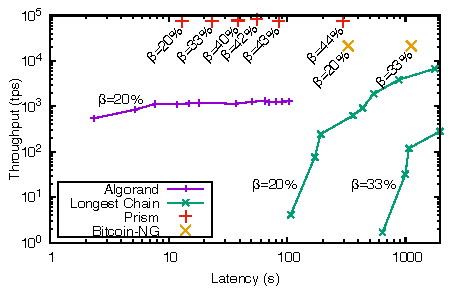
\includegraphics[width=0.75\textwidth]{figures/compare-fig.pdf}
    \caption[Throughput and confirmation latency of Prism, Algorand, Bitcoin-NG, and the longest chain protocol on the same testbed.]{Throughput and confirmation latency of \prism, \algorand, \bng, and the longest chain protocol on the same testbed. Note that the axes are on log scales. For \algorand and the longest chain protocol, parameters are tuned to span an optimized tradeoff between throughput and latency at a given security level. For \bng and \prism, throughput and latency are decoupled so one can simultaneously optimize both at one operating point for a given security level. However, the throughput of Bitcoin-NG drops to that of the longest chain protocol under attack, while that of \prism remains high. More details in \S\ref{sec:related} and \S\ref{sec:eval-performance}. }
    \label{fig:compare}
\end{figure}


In this thesis, we present the design (\S\ref{sec:design}) and  implementation (\S\ref{sec:implementation}) of a Bitcoin-like system based on the \prism consensus protocol. Our implementation features payments as multi-input-multi-output transactions (payments) similar to pay-to-public-key (P2PK) in Bitcoin and Algorand~\cite{algorand, algorandcode}. We evaluate our system on a testbed of up to 1000 EC2 Virtual Machines connected via an emulated wide area network. Figure \ref{fig:compare} summarizes the results. \prism consistently achieves a throughput of over 70,000 tps for a range of security levels $\beta$ denoting the fraction of adversarial compute power.  To guarantee a reversal probability of less than $10^{-9}$, \prism's latency ranges from 13 seconds against an adversary of power $\beta = 20\%$, to $296$ seconds for $\beta = 44\%$. To our knowledge, this makes our system by far the fastest  implementation of a blockchain system with Bitcoin-level security guarantees. Compared to the longest chain protocol, \prism provides about 10,000$\times$ higher throughput and 1,000$\times$ lower latency. Compared to Algorand~\cite{algorand}, the state-of-the-art proof-of-stake system, \prism achieves 70$\times$ the throughput with about 10 seconds higher latency, and can provide a higher level of security  (up to $\beta = 50\%$ vs. $\beta=33\%$ for Algorand).

We make the following contributions:
\begin{itemize}
    \item We implement a Prism client in roughly 10,000 lines of {\tt Rust} code, and quantify its performance in extensive experiments on EC2. Our result validate Prism's core modeling decisions and theory by showing that it can scale both throughput and latency of the longest chain protocol (without compromising security) in a practical setting. Our code is available here~\cite{prismcode}.
    
    \item Our implementation highlights several performance optimizations, e.g., asynchronous ledger updates, and a scoreboarding technique that enables parallel transaction execution without race conditions (see ~\S\ref{sec:implementation-highlights}). We show that with these careful optimizations, it is possible to alleviate CPU performance bottlenecks and provide linear CPU scaling up to at least 8 cores. At this point, the primary bottleneck for our implementation is the underlying database (RocksDB~\cite{rocksdb} and I/O to the SSD persistent storage). This suggests that future research on databases optimized for blockchain-specific access patterns could further improve performance. 
    
    \item We evaluate practical security concerns like censorship attack, balancing attack, and spamming (see ~\S\ref{sec:eval-attack}). Additionally, we propose a simple solution to the spamming problem that reduces spam traffic by 80\% while only adding 5 seconds to the confirmation delay. Our implementation illustrates that \prism performs well even under these attacks, and makes a stronger case for the practical viability of the system.
    
\end{itemize}

%Our implementation and evaluation provide several key takeaways. First, our results validate Prism's core modeling and design decisions in a practical setting by demonstrating that it can scale both throughput and latency of the longest chain protocol independently of one another without compromising the security guarantee. Second, our implementation shows that with careful performance optimization (see ~\S\ref{sec:implementation-highlights}), it is possible to alleviate CPU performance bottlenecks and provide linear CPU scaling up to \ma{XXX cores}. At this point, the primary bottleneck for our implementation is the underlying database (RocksDB~\cite{rocksdb} and I/O to persistent storage (SSDs)). Therefore future research on databases optimized for blockchain-specific access patterns could provide further performance improvements. 


% e.g., asychoronous ledger updates, and a scoreboarding technique that enables parallel transaction execution without race conditions. We show that these optimizations alleviate CPU performance bottlenecks and provide linear CPU scaling, such that the primary bottleneck is the underlying database (RocksDB~\cite{rocksdb} and I/O to persistent storage (SSDs)). Further performance improvements may therefore be possible by optimizing the database.

The rest of the thesis is organized as follows. In \S\ref{sec:related} we discuss different scaling approaches taken in blockchains. In \S\ref{sec:background} we discuss the longest chain protocol and its limitations to motivate the design of the \prism protocol in \S\ref{sec:overview} and \S\ref{sec:design}. We discuss the details of the client implementation with an interface enabling pay-to-public-key transactions in \S\ref{sec:implementation}. Evaluations are presented in \S\ref{sec:eval} to assess the impact of network resources (bandwidth, topology, propagation delay) and computation resources (memory, CPU) on the overall performance. \S\ref{sec:conclusion} concludes the thesis.


%%a host of related topics of core interest to the blockchain ecosystem; this includes interfacing Prism to a smart contract programming layer, introduction of light clients (which are simply interested in making and validating specific transactions) and bootstrapping new Prism clients into a running system - each of these is a future direction of research of great interest.


\if 0

% TODO: do we include performance here? Tell the performance first or explain the protocol first?

% TODO: if to compare the performance, what are the baselines? How to compare (cite numbers, run experiments, if so, do we need to optimize their code?) For some of them, modify Prism client into our impelmentation. For algorand, run their code. But what if their implementation is flawed? Explain the results we got (cause of the bottleneck), understand their bottleneck.

% comparisons: Algorand (fame, it could be that their paper is not doing real transactions. use their real code and try to reproduce the number in the paper), Bitcoin (longest chain), OHIE (parallel chain). Remember to point out the security level. This is FINAL.
% mentions: HotStuff
% Point that Conflux is copy cat
% Use Prism 1.0 to help rationale the protocol in Design section.
% Make other system actually do transactions

% Scale of the evaluation
% Hope that the scalability curves are flat, so that reader can assume the scalability (we could provide a breakdown of the CPU/IO resource spent)

% Mention that we have included all possible functions of the client so it is real.

% TODO: make full use of the code. Change parameters to show the idea of other systems.

Text...

Takeaways from experiments. Maybe insert a figure here. % TODO: possibilities: throughput - latency, different protocols take different positions (curve for parameterized ones)

% other potential comparisons: Conflux, Prism 1.0, Bitcoin-NG



Figure 1: comparison of throughput and latency with other blockchain protocols: 

Algorand - best permissionless PoS BFT protocol

longest chain - the original blockchain protocol (frontier as we vary mining rate and block size)

Ohie - parallel chain protocol (give state execution for free)

Prism - our protocol

Network setting (first draft)

100 nodes

artificial delay 300 ms per hop (exponential)

network bandwidth: whatever is sufficient for Prism to achieve 100K Tps. (around 200 to 300Mbps)


\fi

\section{Related Work}
\label{sec:related}
There are broadly three different approaches to scale the performance of blockchains. First, \textit{on-chain scaling} aims to design consensus protocols with inherently high throughput and low  latency. Protocols such as Bitcoin-NG~\cite{bitcoin-ng}, GHOST~\cite{ghost}, Algorand~\cite{algorand}, OHIE~\cite{ohie} are examples of this approach. 
Second, in \textit{off-chain scaling}, users establish cryptographically-locked agreements called ``payment channels''~\cite{payment-channel} and send most of the transactions off-chain on those channels. 
Lightning~\cite{lightning} and Eltoo~\cite{decker2018eltoo} are examples of this approach. 
Third, \textit{sharding} approaches conceptually maintain multiple ``slow'' blockchains that achieve high performance in aggregate. Omniledger~\cite{kokoris2018omniledger}, Ethereum 2.0~\cite{buterin2016ethereum}, and Monoxide~\cite{monoxide} are examples of this approach. 
These three approaches are orthogonal and can be combined to aggregate their individual performance gains. 
% We also point out that off-chain techniques and sharding are relatively new ideas, and they have not been tested out in the wild like on-chain transactions. 

\if 0
Off-chain solutions offer lower security compared to on-chain solutions; an adversary can open payment channels with many users and simultaneously try to settle old channel balance splits
on the main chain. Because of low throughput on the main chain, only a fraction of these users will be able to defend against this attack by settling their latest channel balance on the main chain.
\gf{what kind of attack do you mean? I don't follow how the attack works.} \vb{I have modified it}
% This can cause a huge loss of funds and trust.
It also requires all the users to be online; if a user goes offline, the channel's other user might settle an old channel balance split.
% going offline for a duration can lead to loss in funds as the  
\pv{Would be good to provide some citations for the statements in this para.}
% Nevertheless, off-chain scaling and sharding techniques introduce new attack vectors and has performance issues in certain types of usage.
Off-chain and sharding transactions are relatively new ideas and they have not been tested out in the wild like on-chain transactions. \ma{I don't think we need to delve into detailed attacks on off-chain solutions. I think you can just say the last sentence: Off-chain and sharding are relatively new.... at the end of the last paragraph, and focus on on-chain in the rest}
%On-chain scaling solutions do not have those problems.
\fi

Since Prism is an on-chain scaling solution, we compare it with other on-chain solutions. 
We explicitly exclude protocols with different trust and security assumptions, like   Tendermint~\cite{kwon2014tendermint},  HotStuff~\cite{yin2019hotstuff}, HoneyBadgerBFT~\cite{miller2016honey}, SBFT~\cite{gueta1804sbft}, Stellar~\cite{stellarsystem}, and Ripple\cite{cachin2017blockchain}, which require clients to pre-configure a set of trusted nodes. 
These protocols target ``permissioned'' settings, and they generally scale to significantly fewer number of nodes than the above mentioned permisionless protocols.
%;  hence we don't directly compared them with \prism.

%\ly{Apart from the permissionless blockchain protocols mentioned above, another class of protocols target the ``permissioned'' settings where the set of nodes participating in the consensus is always fixed. Protocols such as Tendermint~\cite{kwon2014tendermint},  HotStuff~\cite{yin2019hotstuff}, HoneyBadgerBFT~\cite{miller2016honey}, SBFT~\cite{gueta1804sbft} etc fall into this category. We point out that those protocols target different applications and they scale to significantly to a fewer number of nodes than the above mentioned permisionless protocols,  hence we don't directly compared them with \prism.}
%Stellar~\cite{stellarsystem} and Ripple\cite{cachin2017blockchain}, which require clients to pre-configure a set of trusted nodes..


% Those protocols target goals different from a public blockchain like \prism.}
Among protocols with similar security assumptions to ours,  Bitcoin-NG~\cite{bitcoin-ng}  mines blocks  at a low rate similar to the longest chain protocol. In addition, each block's miner continuously adds transactions to the ledger until the next block is mined. This utilizes the capacity of the network between the infrequent mining events, thereby improving throughput, but latency remains the same as that of the longest-chain protocol. Furthermore,  an adversary that adaptively corrupts miners can reduce its throughput to that of the longest chain protocol by censoring the addition of transactions~\cite{parallel}. \prism adopts the idea of decoupling the addition of transactions from the election into the main chain but avoids this adaptive attack. We compare to \bng in \S\ref{sec:eval-performance}.
%We were not able to find an implementation of Bitcoin-NG for use in our experiments.
%\ma{isn't it actually implemented in some projects? be careful about this one; there are 3 cornel profs on pc, and they will know about bitcoin-ng and could talk to Gun Sirer too}
%\ly{bitcoin-ng is implemented (see https://blog.aeternity.com/introduction-to-æternitys-bitcoin-ng-implementation-331d0a1393b4).}

DAG-based solutions like GHOST~\cite{ghost}, Inclusive~\cite{inclusive}, and Conflux~\cite{conflux} were designed to operate at high mining rates, and their blocks form a directed acyclic graph (DAG). 
However, these protocols were later shown to be insecure because they don't guarantee liveness, i.e. the ledger stops to grow, under certain balancing attacks \cite{ghost_attack}. Spectre\cite{spectre} and Phantom \cite{phantom} protocols were built along the ideas in GHOST and Inclusive to defend against the balancing attack, however, they don't provide any formal guarantees. Also, Spectre doesn't give a total ordering and
Phantom has a liveness attack \cite{conflux}.
To the best of our knowledge, the GHOST, Inclusive, Spectre and Phantom protocols have no publicly available implementation, and hence we were not able to compare these protocols with \prism in our performance evaluation. 

The blockchain structure maintained by \prism is also a DAG, but a structured one with a clear separation of blocks into different types with different functionalities (Figure \ref{fig:prism}). 
OHIE~\cite{ohie} and Parallel Chains~\cite{parallel} build on these lessons by running many slow, secure longest chains in parallel, which gives high aggregate throughput at the same latency as the longest-chain protocol. To our knowledge, Parallel Chains has not been implemented. 
In OHIE's latest implementation~\cite{ohiecode}, clients do not maintain the UTXO state of the blockchain and  transactions are signed messages without any context, so it is hard to compare with OHIE in our experiments, where all nodes maintain the full UTXO state.

Algorand~\cite{algorand} takes a different approach by adopting a proof of stake consensus protocol and tuning various parameters to maximize the performance. We compare to Algorand in \S\ref{sec:eval-performance}. Importantly, none of the above protocols simultaneously achieve both high throughput and low latency. 
Their reported throughputs are all lower than \prism's, and their latencies are all higher than \prism's, except for Algorand which has a lower latency.



%%\ma{Should we mention Avalanche?}
%%\vb{Yes. They also claim high throughput and low latency. Currently their protocol is not fully specified in the paper and no implementation available} \ly{one available with only the consensus layer}

%%\ly{TODO: talk about stellar, read algorand's description}

%\ma{One general comment is give credit (generously) if there's an idea in related work that inspired something in prism.}
%\vb{We are inspired by all the DAG approaches. We took the idea of a) changing the main chain rule from GHOST, b) `referencing` blocks from Inclusive, and c) ledger sanitization  from Conflux.}
\chapter{The Longest Chain Protocol}
\label{sec:background}
% In this section, we review Nakamoto's longest chain protocol~\cite{bitcoin} and discuss the fundamental limitations in scaling its latency and throughput. These limitations motivate \prism's design, as we discuss in the next section. 

% %as a natural design to remove these limitations. 
% %%We will explain the design of \prism incrementally, first addressing throughput and then latency.



% \subsection{The longest chain protocol}

The most basic blockchain consensus protocol is Nakamoto's longest chain protocol, used in many systems including \bitcoin and \ethereum.  The basic object is a {\em block}, consisting of {\em transactions} and a reference link to another block. 
%A transaction is a payment signed by a sender's public key, and addressed to a recipient's public key. 
As transactions arrive into the system, a set of nodes, called {\em miners}, construct blocks and broadcast them to other nodes. The goal of the protocol is for all nodes to reach consensus on an ordered log of blocks (and the transactions therein), referred to as the {\em ledger}.

Starting with the {\em genesis} block as the root, each new block mined by a miner is added to create an evolving {\em blocktree}. In the longest chain protocol, honest miners append each block to the leaf block of the longest chain\footnote{In case of variable proof of work, honest miners mine on the ``heaviest chain''.} in the current blocktree, and the transactions in that block are added to the transaction ledger maintained by the blocks in the longest chain. 
A miner earns the right to append a block after solving a cryptographic puzzle, which requires finding a solution to a hash inequality.
 %the leaf block \ma{and the contents of the block being mined?}.  
 The miner includes the solution in the block as a {\em proof of work} (PoW), which other nodes can verify.  The time to solve the puzzle is random and exponentially distributed, with a mining rate $f$ that can be tuned by adjusting the difficulty of the puzzle. How fast an individual miner can solve the puzzle and mine the block is proportional to its hashing power, i.e. how fast it can compute hashes. 
 
 A block is confirmed to be in the ledger when it is $k$-deep in the ledger, i.e. the block is on the longest chain and a chain of $k-1$ blocks have been appended to it. It is proven that as long as the adversary has less than $50\%$ hashing power, the ledger has consistency and liveness properties~\cite{backbone}: blocks that are deep enough in the longest chain will remain in the longest chain with high probability, and honest miners will be able to enter a non-zero fraction of blocks into the ledger. 



\section{Latency Limitation}
\label{s:lc-latency}
A critical attack on the longest chain protocol is the {\em private  double-spend} attack \cite{bitcoin}, as shown in Figure \ref{fig:double_spend}(a). Here, an adversary is trying to revert a block after it is confirmed, by mining a chain in private and broadcasting it when it is longer than the public chain. If the hashing power of the adversary is greater than that of aggregate of the honest nodes, this attack can be easily executed no matter what $k$ is, since the adversary can mine blocks faster on the average than the honest nodes and will eventually  overtake the public chain. On the other hand, when the adversary has less than half the power, the probability of success of this attack can be made exponentially small by choosing the confirmation depth $k$ to be large \cite{bitcoin}. The price to pay for choosing $k$ large is increased latency in confirmation. For example, to achieve a reversal probability of  $0.001$, a depth of $24$ blocks is needed if the adversary has $\beta = 30\%$ of the total hashing power~\cite{bitcoin}.  Figure ~\ref{fig:rd} shows the tradeoff between confirmation depth (and therefore latency) and reliability.

\begin{figure}
\begin{center}
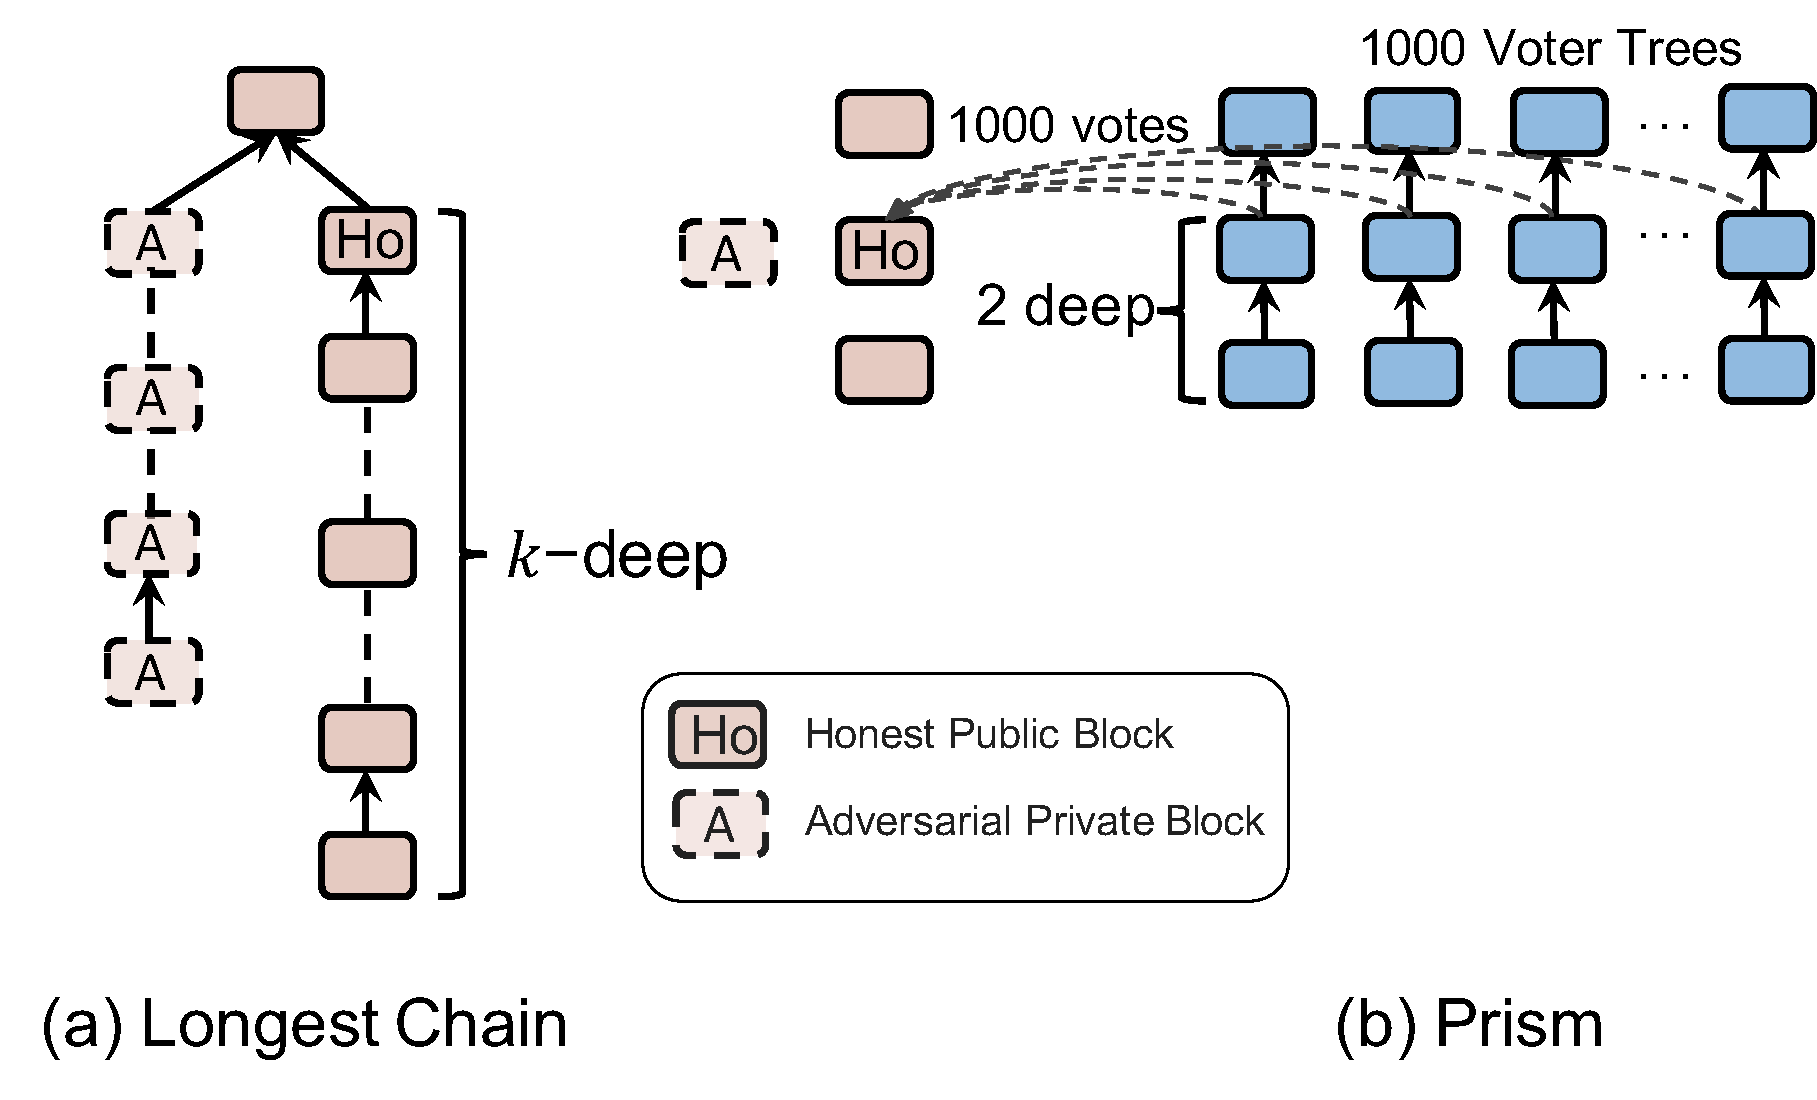
\includegraphics[width=0.75\textwidth]{fast_confirmation_comparision_2.pdf}
\end{center}
    \caption[Depth of confirmation: longest chain vs. Prism.]{Depth of confirmation: longest chain vs. \prism. (a) The longest chain protocol requires a block $Ho$ to be many blocks deep for reliable confirmation, so that an adversary mining in private cannot create a longer chain to reverse block $Ho$. (b) \prism allows each voter block to be very shallow but relies on many voter chains to increase the reliability.}
\label{fig:double_spend}
\end{figure}


%%With Bitcoin's block mining rate of 1 block every 10 minutes, this translates into a latency of 4 hours! Increasing the block mining rate to, say, 1 block per 10 seconds, improves latency to 240 seconds, but the latency to achieve a high level of reliability is still very high. To achieve a reversal probability of $10^{-6}$, a depth of $50$ blocks is required, translating into a latency of $500$ seconds. Figure ~\ref{fig:rd} shows the tradeoff between confirmation depth (and therefore latency) and reliability. \pv{This is a pretty long section and if we are in a space crunch, then its fine to cut a bit.} 

%In Bitcoin, the mining rate is set much more conservatively, a block roughly every 10 minutes, leading to very long confirmation latency. 

%\ma{I've been assuming this figure also shows the reliability-depth tradeoff for Prism?}
% \begin{figure}
%     \centering
%     \begin{subfigure}[b]{\textwidth}
%         \centering
%         \includegraphics[width=0.35\linewidth]{fast_confirmation_comparision_a.pdf}%
%         \hfill
%         \includegraphics[width=0.35\linewidth]{fast_confirmation_comparision_b.pdf}
%     \end{subfigure}
%     \tion{\small Depth of confirmation: longest chain vs. \prism. (a) The longest chain protocol requires a block to be many blocks deep for reliable confirmation, so that an adversary mining in private cannot create a longer chain. (b) \prism allows each voter block to be very shallow but relies on many voter chains to increase the reliability. \ma{please increase the font size of the subfigure labels, or better, separate this into two figures and use latex's subfig environment}} 
% \end{figure}

\begin{figure}
\begin{center}
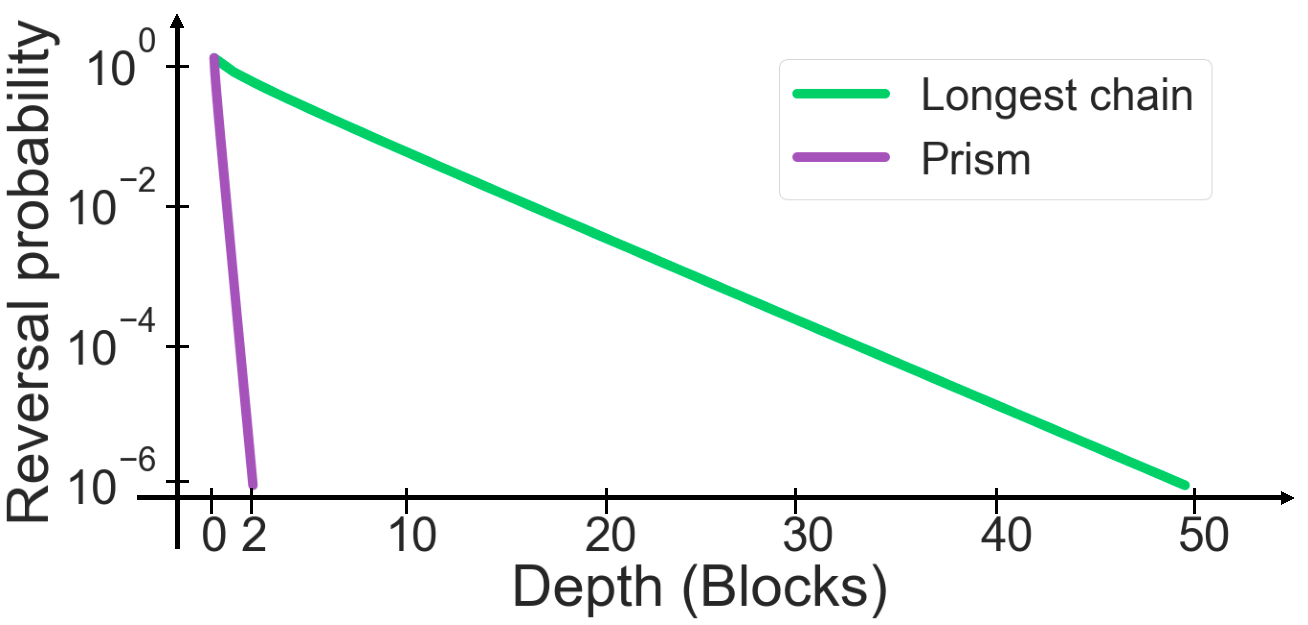
\includegraphics[width=0.6\textwidth]{figures/reliability-depth.pdf}
\end{center}
    \caption[Reliability as a function of confirmation depth.]{\label{fig:rd} Reliability as a function of confirmation depth. The reversal probability of \prism has a factor $m$ improvement over the longest chain protocol in the exponential rate of decrease, where $m$ is the number of voter chains (introduced in \S\ref{sec:overview}).}
\end{figure}
\section{Throughput Limitation}
\label{s:lc-thput}

If $B$ is the block size in number of transactions, then the throughput of the longest chain protocol is at most $fB$ transactions per second (tps). 
However, the mining rate $f$ and the block size $B$ are constrained by the security requirement. Increasing the mining rate increases the amount of {\em forking} of the blockchain due to multiple blocks being mined on the same leaf block by multiple miners within the network delay~$\Delta$. Forking reduces throughput since it reduces the growth rate of the longest chain; recall that only blocks on the longest chain contribute to the ledger. More importantly, forking hurts the security of the protocol because the adversary requires less compute power to overtake the longest chain. In fact, the adversarial power that can be tolerated by the longest chain protocol goes from $50\%$ to $0\%$ as the mining rate $f$ increases \cite{backbone}. 
%(Figure \ref{fig:forking}). 
Similarly, increasing the block size $B$ also increases the amount of forking since the network delay $\Delta$ increases with the block size \cite{decker}.

A back-of-the-envelope calculation of the impact of the forking can be done based on a simple model of the network delay: 
$$ \Delta = \frac{hB}{C} + D,$$
where $h$ is the average number of hops for a block to travel, $C$ is the communication bandwidth per link in transactions per second, and $D$ is the end-to-end propagation delay.  This model is consistent with the linear relation between the network delay and the block size as measured empirically by \cite{decker}. 
%\ma{do we have to mention the possibility of cut-through routing? i think we can skip it and maybe mention it in the discussion section towards the end.}
%\vb{Thats a good idea. There are works (like bloxroute) out there which propose cut-through routing to improve the latency.}
Hence, the utilization, i.e. the throughput as a fraction of the communication bandwidth, is upper bounded by
$$ \frac{fB}{C} < \frac{f\Delta}{h},$$
where $f\Delta$ is the average number of blocks ``in flight'' at any given time, and reflects the amount of forking in the block tree.  %%which is nothing but the \textit{forking rate} on the longest chain. \ma{how is forking rate defined?}
In the longest chain protocol, to be secure against an adversary with $\beta < 50\%$ of hash power, this parameter should satisfy \cite{backbone}
$$f\Delta<\frac{1-2\beta}{\beta}.$$
For example, to achieve security against an adversary with $\beta = 45\%$ of the total hashing power, one needs $f\Delta \approx 0.2$. With $h = 5$, this translates to a utilization of at most $4\%$. The above bound holds regardless of block size; the utilization of the longest chain protocol cannot exceed 4\% for $\beta = 45\%$ and $h=5$.
In summary, to not compromise on security, $f\Delta$ must be kept much smaller than $1$. 
Hence, the security requirement (as well as the number of hops) limits the bandwidth utilization.  

%%$$ \ma{I still don't understand why this is different from the analysis in Appendix %%D.2 of the Prism paper.}
%%\vb{The analysis in D.2 is a conservative necessary condition. Whereas the above %%formula is only a necessary condition. It comes from the simple fact that the %%honest nodes grow at rate $\frac{(1-\beta)}{1+f\Delta}$ and adversary grows at rate %%$f\beta$.}
%%\gf{The phrasing above the equation makes it sound like a necessary condition.} %%\vb{Typo. It is indeed a necessary condition

% \ma{Can we state how security depends on $f\Delta$ here precisely, and replace Figure 3 with one that shows maximum possible $f\Delta$ vs. $\beta$. The next sentence gives the specific point $\beta=0.45$ as an example. The nice thing about this is that it highlights that in the longest chain protocol, to meet the security requirement, one cannot have too many blocks in flight at the same time. Prism doesn't have this limitation. However, if my understanding is correct, it will show that $f\Delta$ can be 1 for $\beta < 0.33$, and drops sharply only for higher security levels. This would mean that the possible utilization for Bitcoin in practice is really $1/h$. Is this correct? Prism can only improve throughput from $1/h$ to $1$, unless we're concerned with very high security?} 
% \vb{The effective throughput due to forking is $fB\big(\frac{1}{1+f\Delta}\big)$} \ly{$f\Delta = \frac{1-2\beta}{\beta}$ See Figure~\ref{fig:forking-new}} \ma{Is this consistent with the Prism theory paper, Appendix D.2? I'm still not happy with our explanation here. My hope is that we can remove Fig. 3, and use the fact that f$\Delta$ must be small for security, and the equation above to show that the utilization of the longest chain protocol is limited. @Vivek: please see if this makes sense and update this section.}


%%In summary, in the longest chain protocol, security of the system is fundamentally at odds with low latency and high throughput. To achieve a low reversal probability, blocks must be deep in the longest chain, increasing confirmation latency. At the same time, increasing the mining rate or block size would compromise security because of forking. As we discuss next, \prism removes these limitations to achieve high throughput, low latency, and security simultaneously. 

%\red{GF: Maybe explain in words why we can hope to fix this problem? The dependency on  graph diameter is fundamental, since all honest nodes have to come to consensus, but the effect of Bitcoin's security requirement could  be circumvented by designing a system that trades latency for communication in its confirmation rule.}

\if 0
\begin{figure}
\begin{center}
\includegraphics[width=0.4\textwidth]{figures/forking_security.pdf}
\end{center}
\caption{ Increasing mining rate or block size increases forking and reduces security. 
\red{GF: Are we going to add numbers to the x-axis? This looks a bit cartoonish, I think having actual nubmers on the axes would help,  if we want to keep this figure at all (not sure it clarifies too much?).} \ly{Shall I redo the plot to put numbers on x-axis and make it the same style as figure 8 to 12?}
\vb{I have added numbers to x-axis for now.}
\gw{Caption says "or block size", but it's not in the figure.}}
\label{fig:forking}
\end{figure}

\fi

% \begin{figure}
% \centering
% \input{figures/fdelta-fig.tex}
% \caption{ Increasing mining rate or block size increases forking and reduces security. \gw{Is this the correct caption for the figure?}} \ma{No. This figure might actually work better with $f\Delta$ on the x-axis. The focus should probably be the region where $f\Delta$ is small, say less than 2 or 3. I'm not sure the figure is correct. @Vivek: please double check} \vb{This figure look correct}
% \label{fig:forking-new}
% \end{figure}






\chapter{Overview of \prism}
\label{sec:overview}

%\ma{I think we need to refer to the Prism theory paper in this section. We are giving the intuition behind the protocol here, but it's important to state that the security properties have been formally proved.}

The selection of a main chain in a blockchain protocol can be viewed as electing a leader block among all the blocks at each level of the blocktree. In this light, the blocks in the longest chain protocol can be viewed as serving three distinct roles: they stand for election to be leaders;  they add transactions to the main chain; they vote for ancestor blocks through parent link relationships. The latency and throughput limitations of the longest chain protocol are due to the {\em coupling} of the roles carried by the blocks. \prism removes these limitations by factorizing the blocks into three types of blocks: proposer blocks, transaction blocks and voter blocks. (Figure \ref{fig:prism}). Each block mined by a miner is randomly sortitioned into one of the three types of blocks, and if it is a voter block, it will be further  sortitioned into one of the voter trees. (Mining is described in detail in \S\ref{sec:mining}).

The proposer blocktree anchors the \prism blockchain. 
Each proposer block contains a list of reference links to transaction blocks, which contains transactions, as well as a single reference to a parent proposer block.
Honest nodes mine proposer blocks on the longest chain in the proposer tree, but the longest chain does not determine the final confirmed sequence of proposer blocks, known as the  \emph{leader sequence}. 
We define the \emph{level} of a proposer block as its distance from the genesis proposer block, and the \emph{height} of the proposer tree as the maximum level that contains any proposer blocks. 
The leader sequence of proposer blocks contains one block at every level up to the height of the proposer tree, and is  determined by the \emph{voter chains}. 

%\gw{Voter tree (blocktree) or voter chain (blockchain)? Since unlike proposer tree, only voter longest chain will participate in voting.}

There are $m$ voter chains, where $m \gg 1$ is a fixed parameter chosen by the system designer. For example, we choose $m=1000$ in our experiments.  The $i$th voter chain is comprised of voter blocks that are mined on the longest chain of the $i$th voter trees. A voter block votes for a proposer block by containing a reference link to that proposer block, with the requirements that: 1) a vote is valid only if the voter block is in the longest chain of its voter tree; 2) each voter chain votes for one and only one proposer block at each level. The leader block at each level is the one which has the highest number of votes among all the proposer blocks at the same level (tie broken by hash of the proposer blocks.) The elected leader blocks then provide a unique ordering of the transaction blocks to form the final ledger. (Ledger formation is explained in detail in \S\ref{sec:confirmation}.)





%%The security of the system rests on the security of the $m$ voter chains, which is guaranteed by longest chain protocol. However, as we discuss next, by relying on many parallel voter chains, \prism significantly reduces the latency required to achieve a desired reversal probability compared to the vanilla longest chain protocol.


\if 0
The voter blocks vote for transactions indirectly by voting for proposer blocks, which in turn link to transaction blocks. Proposer blocks are grouped according to their level in the original block tree \ma{not clear what this means. what is the `original block tree'? does a proposer block have a link to a parent proposer block (this is not shown in the figure)}, and each voter tree votes for exactly one proposer block at each level to select a leader block among them. The leader block is the proposer block which has the highest number of votes among all the proposer blocks at the same level (ties broken by hash of the proposer blocks.) The elected leader blocks can then bring in the transactions to form the final ledger. \ma{Can we explain this more precisely, e.g., To obtain the final ledger, one traverses the elected leader blocks level by level, including the transactions that they link to in order.} The vote from a voter tree is represented by the reference link from a voter block in the longest chains of the voter tree; the longest chains in all the $m$ voter trees maintain the security of the whole system, as explained next.

\fi

%\begin{figure}
%    \centering
%    \tikzstyle{proposer} = [draw, fill=blue!20, rectangle, rounded corners, minimum height=1em, minimum width=1.6em, text centered]
\tikzstyle{voter} = [draw, fill=green!20, rectangle, rounded corners, minimum height=1em, minimum width=1.6em]
\tikzstyle{transaction} = [draw, circle, fill=yellow!20]

% The block diagram code is probably more verbose than necessary
\begin{tikzpicture}[auto, node distance=0.8cm,>=latex']
\node [proposer] (p0l) {\tiny L};
\node [proposer, below of=p0l] (p1l) {\tiny L};
\node [proposer, left=0.1cm of p1l] (p1s) {};
\node [proposer, below of=p1l] (p2l) {\tiny L};
\node [proposer, right=0.1cm of p2l] (p2s) {};
\node [proposer, below of=p2l] (p3l) {\tiny L};

\node[transaction, above left = 0.01cm and 0.45cm of p0l] (t00){};
\node[transaction, below right = 0.06cm and 0.02cm of t00] (t01){};
\node[transaction, left = 0.25cm of p1s] (t10){};
\node[transaction, above right = 0.07cm and 0.02cm of t10] (t11){};
\node[transaction, below right = 0.10cm and 0.07cm of t10] (t12){};
\node[transaction, below left = 0.05cm and 0.25cm of p2l] (t20){};
\node[transaction, above left = 0.07cm and 0.13cm of t20] (t21){};
\node[transaction, left = 0.35cm of p3l] (t30){};
\node[transaction, above left = 0.05cm and 0.11cm of t30] (t31){};
\node[transaction, left = 0.25cm of t30] (t32){};
\draw[densely dashed, <-] (t00)  to [looseness=0.4] (p0l);
\draw[densely dashed, <-] (t01)  to [looseness=0.4] (p0l);
\draw[densely dashed, <-] (t10)  to [looseness=0.4] (p1l);
\draw[densely dashed, <-] (t11)  to [looseness=0.4] (p1l);
\draw[densely dashed, <-] (t12)  to [looseness=0.4] (p1l);
\draw[densely dashed, <-] (t20)  to [looseness=0.4] (p2l);
\draw[densely dashed, <-] (t21)  to [looseness=0.4] (p2l);
\draw[densely dashed, <-] (t30)  to [looseness=0.4] (p3l);
\draw[densely dashed, <-] (t31)  to [looseness=0.4] (p3l);
\draw[densely dashed, <-] (t32)  to [looseness=0.4] (p3l);


\node [voter, right=1cm of p0l] (v00) {};
\node [voter, below of=v00] (v01) {};
\node [voter, below of=v01] (v02) {};
\node [voter, below of=v02] (v03) {};
\draw[<-] (v00) to (v01);
\draw[<-] (v01) to (v02);
\draw[<-] (v02) to (v03);

\node [voter, right=0.3cm of v00] (v10) {};
\node [voter, below of=v10] (v11) {};
\node [voter, below of=v11] (v12) {};
\node [voter, below of=v12] (v13) {};
\draw[<-] (v10) to (v11);
\draw[<-] (v11) to (v12);
\draw[<-] (v12) to (v13);

\node [right=0.3cm of v10] (space0) {$\cdots$};
\node [below of=space0] (space1) {$\cdots$};
\node [below of=space1] (space2) {$\cdots$};
\node [below of=space2] (space3) {$\cdots$};

\node [voter, right=0.3cm of space0] (v20) {};
\node [voter, below of=v20] (v21) {};
\node [voter, below of=v21] (v22) {};
\node [voter, below of=v22] (v23) {};
\draw[<-] (v20) to (v21);
\draw[<-] (v21) to (v22);
\draw[<-] (v22) to (v23);

\draw[densely dashed, <-] (p0l)  to [looseness=0.3] (v00);
\draw[densely dashed, <-] (p1l)  to [looseness=0.3] (v01);
\draw[densely dashed, <-] (p2l)  to [looseness=0.3] (v02);
\draw[densely dashed, <-] (p3l)  to [looseness=0.3] (v03);

\draw[densely dashed, <-] (p0l)  to [looseness=0.3] (v10);
\draw[densely dashed, <-] (p1l)  to [looseness=0.3] (v11);
\draw[densely dashed, <-] (p2l)  to [looseness=0.3] (v12);
\draw[densely dashed, <-] (p3l)  to [looseness=0.3] (v13);

\draw[densely dashed, <-] (p0l)  to [looseness=0.3] (v20);
\draw[densely dashed, <-] (p1l)  to [looseness=0.3] (v21);
\draw[densely dashed, <-] (p2l)  to [looseness=0.3] (v22);
\draw[densely dashed, <-] (p3l)  to [looseness=0.3] (v23);

\end{tikzpicture}
%    \caption{\prism: Factorizing the blocks into three types of blocks: proposer blocks, transaction blocks and voter blocks. \ma{can we increase the font size a bit?} }
%    \label{fig:prism}
%\end{figure}

\begin{figure}
\begin{center}
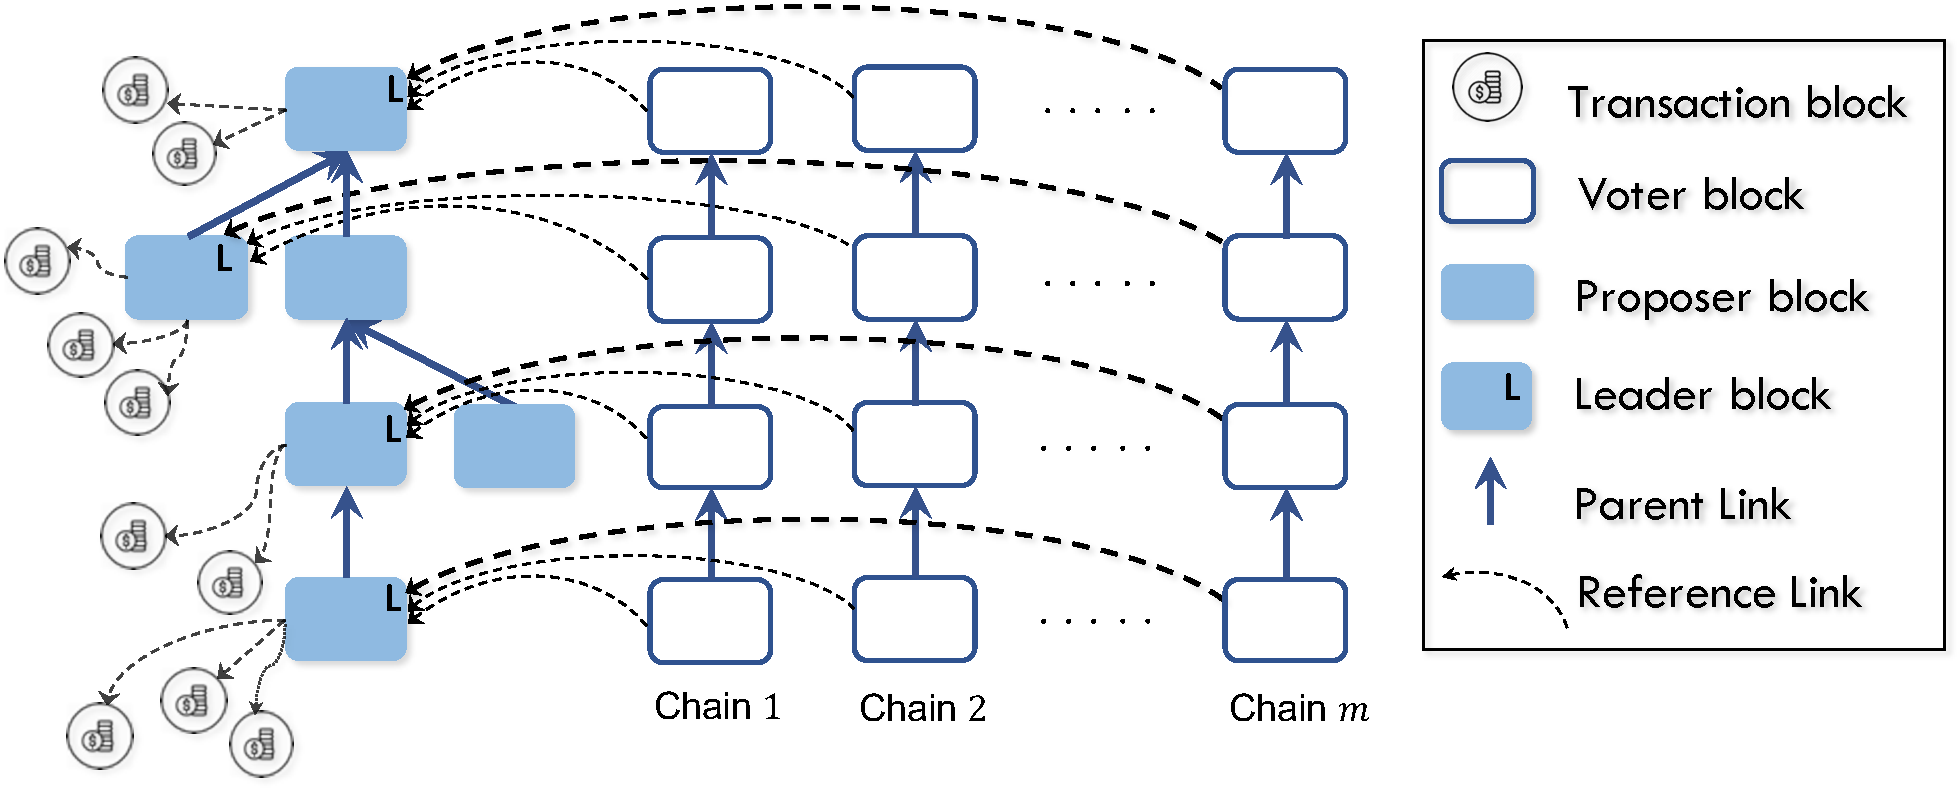
\includegraphics[width=0.45\textwidth]{figures/Prism_main.pdf}
\end{center}
\vspace{-2mm}
\caption{\small \prism: Factorizing the blocks into three types of blocks: proposer blocks, transaction blocks and voter blocks.}
\label{fig:prism}
\vspace{-5mm}
\end{figure}

%%Thus, the parent links in the original block tree have two implicit functionalities which are explicitly separated in this representation: 1) they provide a partial ordering of the proposal blocks according to their levels, and 2) they allow blocks to vote for each other. 
% they help the voting blocks to vote for each other.
%%\blue{It's unclear here what is meant by having a block ``support" another block.}

\if 0

\section{Security Model}
\vb{Let $\mathcal{N}$ denote  the nodes in the system and with of loss of generality, we assume each node has equal mining power. Let $\mathcal{H} \subseteq \mathcal{N}$ denote the set of honest nodes and $\mathcal{N} \setminus \mathcal{H}$ is set the adversarial nodes. The fraction of adversarial nodes, $\beta = 1 - \frac{|\mathcal{H}|}{|\mathcal{N}|}$, is assumed to be less then $0.5$. 
%We assume a network model where the delay for a block of size $B$ is equal to $\Delta = \frac{B}{C}+D$, where $B/C$ is the processing delay and $D$ is the propagation delay.
%We model the protocol as running in rounds where each round is of duration equal to the delay ($\Delta$) corresponding to the largest sized block in the \prism protocol. 
The adversarial nodes do not have to follow the \prism protocol - they can mine new blocks with any content and anywhere on the blockchain, and  unlike honest users, they can keep their mined block in private and release it anytime in future. 
%c) their action in a given round is a function of the action of the honest nodes up to and including that round.
However, the adversary cannot perform certain actions such as modifying the block content of blocks mined by honest nodes or withholding blocks mined by an honest node from reaching other honest nodes.
}

\fi

\section{Security and Latency}
\label{sec:prism-latency}

%The ledger is maintained by the leader proposer blocks at all the levels. 

The votes from the voter trees secure each leader proposer block, because changing an elected leader requires reversing enough votes to give them to a different proposer block in that level. 
Each vote is in turn secured by the longest chain protocol in its voter tree. If the adversary has less than $50\%$ hash power, and the mining rate in each of the voter trees is kept small to minimize forking,  then the consistency and liveness of each voter tree guarantee the consistency and liveness of the ledger maintained by the leader proposer blocks. 
However, this would appear to require a long latency to wait for each voter block to get sufficiently deep in its chain. What is interesting is that when there are many voter chains, the same guarantee can be achieved without requiring each and every vote to have a very low reversal probability, thus drastically improving over the latency of the longest chain protocol. 


To get some intuition, consider the natural analog of the private double-spend attack on the longest chain protocol in \prism. Figure \ref{fig:double_spend}(b) shows the scenario. An honest proposer block $Ho$ at a particular level has collected votes from the voter chains. Over time, each of these votes will become deeper in its voter chain. An attack by the adversary is to mine a private proposer block $A$ at the same level, and on each of the voter trees, fork off and mine a private alternate chain and send its vote to block $A$. After leader block $Ho$ is confirmed, the adversary continues to mine on each of the alternate voter chains to attempt to overtake the public longest chain and shift the vote from $Ho$ to $A$. If the adversary can thereby get more votes on $A$ than on $Ho$, then its attack is successful. The question is how deep do we have to wait for each vote to be in its voter chain in order to confirm the proposer block $Ho$?

Nakamoto's calculations will help us answer this question. As an example, at tolerable adversary power $\beta = 30\%$, the reversal probability in a single chain is $0.45$ when a block is $2$-deep \cite{bitcoin}. With $m=1000$ voter chains and each vote being $2$-deep, the expected number of chains that can be reversed by the adversary is $450$. The probability that the adversary can get lucky and reverse more than half the votes, i.e. $500$, is about  $0.001$. Hence to achieve a reversal probability, $\epsilon = 0.001$, we only need to wait for the votes to be  $2$-deep, as opposed to the $24$ block depth needed in the longest chain protocol (\S\ref{s:lc-latency}). This reduction in latency comes without sacrificing security: each voter chain can operate at a slow enough mining rate to tolerate $\beta$ adversarial hash power. Furthermore, increasing the number of voter chains can further improve the confirmation reliability without sacrificing latency; for example, doubling the number of voter chains from $1000$ to $2000$ can reduce the reversal probability from $0.001$ to $10^{-6}$.

We have discussed one specific attack, focusing on the case when there is a single public proposer block on a given level. Another possible attack is when there are two or more such proposer blocks and the adversary tries to balance the votes between them to delay confirmation. It turns out that the attack space is quite huge and these are formally analyzed in \cite{prism-theory} to obtain the following guarantee on the confirmation latency, regardless of the attack:

 \begin{theorem}[Latency, Thm. 4.8 \cite{prism-theory}] \label{cor:latency_fast}
For an adversary with $\beta< 50\%$ of hash power, network propagation delay $D$, \prism with $m$ chains confirms  \textit{honest}\footnote{Honest transactions are ones which have no conflicting double-spent transactions broadcast in public.} transactions at reversal probability $\epsilon$ guarantee with latency upper bounded by
\begin{equation}
\label{eq:latency}
 Dc_1(\beta) +  \frac{Dc_2(\beta)}{m} \log \frac{1}{\epsilon}\;\; \text{ seconds},
\end{equation}
where $c_1(\beta)$ and $c_2(\beta) $ are $\beta$ dependent constants.
\end{theorem}

For large number of voter chains $m$, the first term dominates the above equation and therefore Prism achieves near optimal latency, i.e. proportional to the propagation delay $D$ and independent of the reversal probability. Figure \ref{fig:rd} compares the latency-reliability tradeoffs of \prism and the longest chain protocol. Note that (\ref{eq:latency}) is a worst-case latency bound that holds for {\em all} attacks. In Section \ref{sec:balancing}, we will evaluate the latency of our system under the balancing attack. 


\section{Throughput}
\label{sec:thruput}

To keep \prism secure, the mining rate and the size of the voter blocks have to be chosen such that each voter chain has little forking. The mining rate and the size of the proposer blocks have to be also chosen such that there is very little forking in the proposer tree. Otherwise, the adversary can propose a block at each level, breaking the liveness of the system. Hence, the throughput of \prism would be as low as the longest chain protocol if transactions were carried by the proposer blocks directly. 


To decouple security from throughput, transactions are instead carried by separate transaction blocks. Each proposer block when it is mined refers to the transaction blocks that have not been referred to by previous proposer blocks. This design allows throughput to be increased by increasing the mining rate of the transaction blocks, without affecting the security of the system. The throughput is only limited by the computing or communication bandwidth limit $C$ of each node, thus potentially achieving $100\%$ utilization. In contrast, as we discussed in \S\ref{s:lc-thput}, the throughput of the longest chain protocol is security-limited, resulting in low network utilization. \cite{prism-theory} formally proves that \prism achieves near optimal throughput:

\begin{theorem}[Throughput, Thm. 4.4\cite{prism-theory} ]
\label{thm:throughput} For an adversary with $\beta < 50\%$ fraction of hash power and network capacity C, Prism can achieve  $(1-\beta)C$ throughput and maintain liveness in the ledger.
\end{theorem}

%Note that the reference links from a proposer block to its transaction blocks are sealed in the proof-of-work of the proposer block. Hence, once a proposer block is mined, there is no way for an attacker to change the reference links to the transaction blocks. In contrast, the transactions that a miner in \bitcoin-NG adds onto the ledger after its block enters the main chain are {\em not} sealed by the proof-of-work. Hence, \bitcoin-NG is susceptible to censorship attacks.

\smallskip
\noindent{\bf Remark on security model:} The Prism theory paper~\cite{prism-theory} analyzed the protocol in a synchronous round-based network model under standard assumptions about the adversary. In particular, the delay for a block of size $B$ was assumed to be equal to $\Delta = \frac{B}{C}+D$, where $B/C$ is the processing delay and $D$ is the propagation delay, and the protocol was assumed to run in rounds where each round is of duration equal to the delay ($\Delta$) corresponding to the largest sized block. The adversarial nodes do not have to follow protocol - they can mine new blocks with any content and anywhere on the blockchain, and  unlike honest users, they can keep their mined blocks in private and release them at anytime in the future. However, the adversary cannot modify the content of blocks mined by honest nodes or withhold blocks mined by an honest node from reaching other honest nodes. Refer to \S2 of~\cite{prism-theory} for the full specification of the model. This model does not capture the impact of artifacts like queuing delay or asynchronous communication on performance. Nevertheless our implementation shows that the overall performance characteristics predicted by the theory hold in a practical setting. 


% To decouple security from throughput, transactions are instead carried by separate transaction blocks. The transaction blocks enter into a pool after they are mined. Each proposer block when it is mined refers to the transaction blocks in the pool that have not been referred to by previous proposer blocks. When a proposer block is confirmed to be the leader of its level, the transactions in all the transaction blocks it refers to enter into the ledger. \ma{The last three sentences could be cut from here and discussed in the design section} The throughput of the system can be increased by increasing the mining rate of the transaction blocks, without affecting the security of the system. This throughput is only limited by the computing or communication bandwidth limit $C$ of each node, thus potentially achieving $100\%$ utilization. In contrast, as we discussed in \S\ref{s:lc-thput}, the throughput of the longest chain protocol is security-limited, resulting in low network utilization. 





%\ma{If we include the figure I mentioned at the end of 2.1, which shows the relationship between $f\Delta$ and security, then we can recall that in the section and explain that transaction blocks overcome this problem}


%%Show that Prism is the optimal (theory). See Fig.~\ref{fig:protocols-comparison}. Optimal in terms of communication limit. But the implementation is limited by state execution. Compare to Hotstuff. 



% \subsection{Formal guarantees}
% The results established about the \prism protocol in a recent theoretical paper~\cite{prism-theory} provide the following throughput and latency guarantees. \ly{update the bib file to reflect that the paper has been published. also consider anonymous issues}




% The above two results show that of Prism achieves near optimal throughput and latency.

% \ma{@Vivek: please summarize the main results from the theory paper here.}
% \vb{done.}



\if 0

\begin{figure}
\begin{center}
\includegraphics[width=0.4\textwidth]{chains-table.jpg}
\end{center}
\caption{\label{fig:protocols-comparison} Table: Comparison }
\end{figure}

\fi

\chapter{Design}
\label{sec:design}

% \vb{ A possible notation is to use capital letters for tuples and small letters otherwise. Header $H$, Content $C$, Block $B=(H,C)$.
% $H=(P,n,D)$, $P$ is the content, $n$ is nonce and $D$ is $\texttt{digest}(C)$.
% Tx block $B^T$, Tx header $H^T$, Tx parent $P^T$, Tx digest $D^T$ and Tx content $C^T$ (similar for prop. and voter block). $B \in \{B^T, B^P, B^V\}$ and so on..}

\section{Notation}
\label{sec:blocktypes}
Each block $B=(H,C)$ is a tuple containting a header $H$ and content $C$.
As discussed in  \S\ref{sec:overview}, there are three types of blocks: transaction blocks, proposer blocks,  and voter blocks.
In all three types, the header $H=(P, n, D)$ is a tuple containing: (1) the hash $P$ of the parent block,
%(\vb{conceptually parent blocks also differ}) \ma{seems ok to me} 
(2)  a valid PoW nonce $n$, and (3) a content digest $D=\texttt{Digest}(C)$. % proving that the block was mined in the correct category (transaction, proposer, or voter). 
We add a superscript to the above notations to denote the type of block being referred. 
For example, we refer  to proposer blocks by $B^P$, transaction blocks by $B^T$, and voter blocks by $B^V$.
% Along the same lines, a proposer block's header, content, and parent are denoted by $H^P$, $C^P$, and $P^P$, respectively, and its content digest by $D^P$.

% The nonce $n$ and content digest $D$ are explained further in the mining procedure (\S\ref{sec:mining}).

%\todo{I intentionally did not  describe what is actually done in the code w.r.t. parent blocks because I think it may confuse people more. Let me know what you think.}
% \ma{I think this is at the right level}

%\paragraph{Transaction blocks.}
% \smallskip
% \noindent{\bf Transaction blocks.}
% Transaction blocks do not need a parent block,  so  $P^T=\emptyset$.
% The content of a transaction block is an ordered list of transactions: $C^T := [t_1, \ldots, t_m]$.
% drawn from the miner's local a memory pool \texttt{mempool} of transactions that have not yet been  incorporated into a transaction block.
% Note that a transaction $t$ is a payment from a sender's public key to a recipient's public key, signed by the sender. 
% \gw{Do we want to mention about multiple senders and recipients?}


% They contain a list of transactions, and a pointer to a parent proposer block. \ma{why do transaction blocks need a pointer to a proposer block? this is also not shown in in Fig. 4} \ma{It might be useful to define a transaction, e.g., it is a payment from a sender public key to a recipient public key, signed by the sender}

% \vb{Below we have described both the content and the mining procedure of the proposer and voter blocks. We can explicitly state that perhaps} \ma{I think this is ok} 

% \smallskip
% \noindent{\bf Proposer blocks.}
% Since the proposer tree is built in a longest-chain fashion, proposer blocks choose as their parent $P^P$  the tip of the longest chain in the proposer tree. 
% Each proposer block's content, $C^P$, is an ordered list of references to other proposer and/or transaction blocks.  
% We compute $B$'s set of \emph{ancestors} by following the chain of parent links in the proposer tree.
% For proposer block $B$, let $C^P_1 =[B^P_{i_1}, B^P_{i_2}, \ldots]$ denote an ordered list of proposer blocks that are neither indirectly referenced or among content of $B$'s ancestors.
% Let $C^P_2 = [B^T_{j_1}, B^T_{j_2},\ldots]$ denote an ordered list of transaction blocks that are not referenced (directly or indirectly) by any of $B$'s ancestors or by any of the proposer blocks in $C^P_1$.
% The content of the proposer block is the concatenation of these two ordered lists: $C^P  :=(C^P_1, C^P_2)$.
% Note that $C^P$ actually stores references to the listed blocks, but we describe them as blocks here to reduce notation.
% Honest nodes mine proposer blocks on the longest chain in the proposer blocktree, but the longest chain does not determine the final confirmed sequence of proposer blocks, known as the  \emph{leader sequence}. 
% We define the \emph{level} of a proposer block as its distance from the genesis block (Figure \ref{}), and the \emph{height} of the proposer tree as the maximum level that contains any proposer blocks. 
% The confirmed leader sequence of proposer blocks contains one block at every level up to the height of the proposer blocktree, and is  determined by the \emph{voter trees}. 
% \smallskip
% \noindent{\bf Voter blocks.}
% There are $m$ voter trees, where $m \gg 1$ is a fixed parameter chosen by the system designers. 
% The $i^{th}$ voter tree is comprised of voter blocks that are mined on the longest chain of the voter tree. 
% Voter trees are also  built in a longest-chain fashion,  so for a voter block  $B^{V_i}$ in the $i^{th}$ voter tree,  its parent $P^{V_i}$ is the tip of the longest chain in the $i^{th}$ voter tree.
% The block's contents $C^{V_i}$ are a list of references to proposer blocks, or \emph{votes}.
% Recall that the \emph{level} of a proposer block denotes its distance from the genesis block, and the \emph{height} $h$ of the proposer tree is the maximum level that contains any proposer blocks.
% Let $L=\{1,\ldots, h\}$ denote the set of all levels in the proposer blocktree.
% Voter trees are built in a longest-chain fashion; each voter tree's longest chain is allowed to vote at most once on any level in  $L$.
% For a voter block $B^V$, let $\ell'_{B}$ be the latest level of proposer block voter by $B^V$'s ancestors and thus $B^V$ has to vote on levels $\{\ell'_{B}+1,\cdots,h\}$.
% % let $L'_{B}$ denote the set of levels that have already been voted on by $B$'s ancestors. (\vb{$L'_{B}$ is a continuous set. To simplify the notation we can say that `for voter block $B$, let $\ell'_{B}$ be the latest level of proposer block voter by $B$'s ancestors and thus $B$ has to vote on levels $\{\ell'_{B}+1,\cdots,h\}$})
% % Let $L_{B} = L \cap L'_{B}$ be the set of remaining levels, and let $\mathcal P_i$ denote the set of proposer blocks at level  $i$. \gw{You mean $L - L'_B$?}
% The content of the voter block, $C^V := [B^P_{\ell'_{B}+1},\ldots,B^P_{h}]$ is a list of proposer blocks where with some abuse of notation, $B^P_{\ell}$ denotes a vote for  (pointer to) a proposer block at level $\ell$. 
% In words,  the voter block contains a list of one vote per unvoted level in the block's ancestor list. 
% \ma{It seems we can simplify this description per Vivek's suggestion} \vb{done}
% this list includes at most one pointer to a proposer block at every level of the proposer blocktree that has not yet been voted on by any of $B$'s ancestors in the $i$th voter tree. 
% We call such a pointer a \emph{vote}, since it is effectively endorsing a given proposer block. 
% In other words, each voter tree is allowed  at most one vote for each level of the proposer tree, where only the votes contained in the longest chain of each voter tree are counted. 
% We explain how these votes are used to confirm transactions in Section \ref{sec:confirmation}


% \todo{Mention database, mempool, etc. data structures as well. These will be discussed in more detail in the Implementation subsection, but we just explain what they are here so that the pseudocode makes sense. }

% \subsection{Protocol}
% The protocol has two primary components: mining and ledger formation. 

% \ma{One thing that would be good to mention is that the lists in the different blocks have bounded length. Perhaps discuss how a block picks among its options when the list doesn't fit everything.}
% \vb{The list of different blocks will vary in length but for simplicity we can leave it unbounded. In expectation, the size of the list is $1$.}

\section{Mining}
\label{sec:mining}
Miners should not be able to choose \emph{a priori} which type of block they are mining; this is essential for the security of the scheme, since otherwise the adversary could concentrate all  of its power on a subset of block trees and overpower them. 
\emph{Cryptographic sortition} is used to ensure that miners cannot choose which type of block they mine.
Nodes simultaneously mine one transaction block, one proposer block, and $m$ voter blocks (one for each tree). 
Only after a valid proof of work is found does the miner learn if the mined block is a transaction, proposer, or voter block. 
The mining process has three steps (four including validation): 

\noindent \textbf{(1) Superblock generation.} 
When a miner starts mining, it creates a \emph{superblock} that simultaneously contains the parents and contents for all $m+2$ possible sub-blocks (1 transaction sub-block, 1 proposer, and $m$ voter sub-blocks). The parents and contents differ for each type of block.
This superblock is updated whenever the miner receives a new network message that changes either the header or the content of any of the sub-blocks. 

\emph{Transaction sub-block $B^T$:} 
%The miner chooses a parent $R_{B^T}$ as described in Section  \ref{sec:blocktypes}. 
Transaction blocks do not need a parent block,  so  $P^T=\emptyset$.
The content of a transaction block, $C^T$, is an ordered list of transactions,  drawn from a data structure similar to the Bitcoin \texttt{mempool}, except in Bitcoin, \texttt{mempool} stores all transactions that have not yet been included in the main chain; in Prism, once a transaction is included in a valid transaction block, it is permanently removed from the \texttt{mempool}.
This is because the transaction block (hence its contained transactions), is guaranteed to eventually be included in the ledger (\S\ref{sec:confirmation}).
Upon receiving a new transaction block over the network, the miner should remove the transactions in the new block from its own mempool and transaction block content. 

\emph{Proposer sub-block $B^P$:} 
Proposer tree is built in a longest-chain fashion; proposer blocks choose as their parent $P^P$  the tip of the longest chain in the proposer tree. 
Each proposer block's content, $C^P  :=(C^P_1, C^P_2)$, is an ordered list of references to other proposer and transaction blocks, where
$C^P_1$ is an ordered list of proposer blocks that are neither referenced nor among content of $B^P$'s ancestor block\footnote{ Ancestor blocks are computed by following the chain of links from $B^P$ in the prop. tree.}, and
 $C^P_2$ is an ordered list of transaction blocks that are not referenced (directly or indirectly) by any of $B^P$'s ancestors or by any of the proposer blocks in $C^P_1$.
% Note that $C^P$ actually stores references to the listed blocks.
A miner updates content $C^P$ upon receiving a new transaction block or a new proposer block. 
% The miner chooses a parent $P^P$ and block contents $C^P$ as described in  \S\ref{sec:blocktypes}. 
% That  is, miners store a list of references to proposer and transaction blocks that have not been referenced by any other proposer blocks in $B^P$'s ancestry. 
% In the former case, it can choose to add a reference to the new transaction block to the miner's proposer block content.
% In the latter case, if the newly-received proposer block is at the same level as the miner's in-progress block, the miner should update the in-progress proposer block's parent so as to extend the longest chain and also update the content $C^P$.
%(\vb{and the content?)} \ma{yep, i think it should be `parent and content'}. 

\emph{Voter sub-block $B^{V_i}$ in the $i^{th}$ voter tree:} 
Voter trees are also  built in a longest-chain fashion; the  parent of voter block  $B^{V_i}$, $P^{V_i}$, is the tip of the longest chain in the $i^{th}$ voter tree.
The content, $C^{V_i}$, is a list of references to proposer blocks, or \emph{votes}.
% , and the \emph{height} $h$ of the proposer tree is the maximum level that contains any proposer blocks.
Each voter tree's longest chain is allowed to vote at most one proposer block on any level\footnote{
Level of a proposer block is its distance from the genesis block.} of the proposer tree.
Let $h$ denote the last level in the proposer blocktree and $\ell_B$ denote the last level voted by $B_{V_i}$'s ancestors.
% For a voter block $B^{V_i}$, let $\ell'_{B}$ be the latest level of proposer block voter by $B^{V_i}$'s ancestors and thus $B^{V_i}$ has to vote on levels $\{\ell'_{B}+1,\cdots,h\}$.
% let $L'_{B}$ denote the set of levels that have already been voted on by $B$'s ancestors. (\vb{$L'_{B}$ is a continuous set. To simplify the notation we can say that `for voter block $B$, let $\ell'_{B}$ be the latest level of proposer block voter by $B$'s ancestors and thus $B$ has to vote on levels $\{\ell'_{B}+1,\cdots,h\}$})
% Let $L_{B} = L \cap L'_{B}$ be the set of remaining levels, and let $\mathcal P_i$ denote the set of proposer blocks at level  $i$. \gw{You mean $L - L'_B$?}
Then the content of the voter block $B^{V_i}$ is $C^V := [B^P_{\ell'_{B}+1},\ldots,B^P_{h}]$, list of proposer blocks where with some abuse of notation, $B^P_{\ell}$ denotes a vote for  (pointer to) a proposer block at level $\ell$. 
In words,  the voter block contains a list of one vote per unvoted level in the block's ancestors. 

% The miner chooses a parent $P^{V_i}$ as described in   \S\ref{sec:blocktypes}. 
% Its content $C^{V_i}$  is references to one proposer block on each level that have not yet been voted on by any of its ancestors. 
% \ma{Feels a bit repetitive with 4.1, but i think it's OK}
By default, nodes will vote for the first proposer block they see at a given level.
Notice that the content $C^{V_i}$ is updated if the miner receives either a new proposer block at a previously-unseen level or a new voter block for the $i^{th}$ tree that changes the longest chain of that voter tree. 
In  the former case, the miner adds a vote for that level. 
In the latter case, the miner updates its parent block $P^{V_i}$ so as to extend the longest chain and also updates the content $C^{V_i}$.
All the contents and parent links are concatenated into a superblock $B=(H,C)$ with header 
$H=(P:=[P^T,  P^P, P^{V_1}, \ldots, P^{V_m}], n, D)$ 
% \ma{nit. do we need the $\emptyset$?} \vb{nope..}
and content 
$ C := [ C^T, C^P, C^{V_1}, \ldots, C^{V_m}]$.
The content digest $D$ is explained next.


\noindent \textbf{(2) PoW and sortition.}
Once the superblock is formed, the miner mines by searching for a nonce $n$ such that $Hash( H)\leq q$, where $Hash(\cdot)$ denotes a hash function, and $q$ denotes a difficulty threshold. 
For a one-way hash function, the miner can do no better than brute-force search, so it cycles through difference values of nonces $n$ until  finding one such that $Hash(H) \leq q$. Upon finding a valid nonce,  sortition  occurs. 
We divide the numbers from $0$ to $q$ into regions corresponding to different block types. 
For example, $[0,q_T]$ denotes a transaction block, $[q_T+1,q_P]$ denotes a  proposer block, and $[q_P+1,q]$ denotes voter blocks,  split evenly into  $m$ regions, one per voter tree.
The output region of $Hash(H)$ determines the block type.


\noindent \textbf{(3) Block pruning.}
Passing around a large superblock after mining would waste unnecessary bandwidth. 
Hence, to improve space efficiency, instead of using the full concatenated parent block and content lists, only the relevant content is retained after mining and the type of the block is known.
For example, a mined proposer block would contain only the proposer parent reference , $P^P$, and proposer content, $ C^P$; it would \emph{not} store transactions or votes.
However,  if we do this naively, block validators would not be able to tell if the cryptographic sortition was correctly executed.
To address this, we alter our header to contain the following:
$H=\left(\textsf{MerkleRoot}(P), n, D := \textsf{MerkleRoot}(C)\right)$, 
 where $\textsf{MerkleRoot}(\cdot)$ denotes the Merkle root of a Merkle tree \cite{merkle} 
%  \ma{cite something for Merkle tree} 
generated from the contained array.
%To avoid the overhead of including all $m+2$ parents and content hashes in every block, Prism block headers contain: a) the Merkle root of a tree with $m+2$ parent blocks, b) the Merkle root of a tree with $m+2$ contents, and c) a nonce. \gw{"a)" is different from our implementation. In implementation, every block has a proposer parent. And every voter block has a voter parent which is stored inside content.}
%Upon finding a valid nonce, the hash of the block deterministically determines if the block is a proposer block, a transaction block, or a voter block on one  of the $m$ voter trees.  
%The mined, sortitioned block includes a header, the appropriate parent and content for the soritioned block type, and the respective Merkle proofs.
In addition to the pruned content and header, we include \textit{sortition proofs}, Merkle proofs attesting to the fact that the block  was mined correctly.
In our proposer block example, the Merkle proof would include the sibling node for every  node in the path from the proposer content $C^P$ to the root $\textsf{MerkleRoot}(C)$ in the Merkle tree. 
Hence $\textsf{MerkleProof}( C)$ (resp. $\textsf{MerkleProof}(P)$) is an array of  size $\log_2 (m)$ -- a primary source of storage overhead in Prism blocks. 


\noindent \textbf{(4) Block validation.}
Upon  receiving a mined Prism block $B=(H,C)$, a validator checks two things. 
First, it  checks that $Hash( H) \leq q$ and that the cryptographic sortition is correct  (i.e., that the hash  maps to the correct region for the block type).
Next, it checks the sortition proof.  
To do this, it takes content $C$ (resp. parent) in  the block, and ensures that the Merkle proof validation gives the content (resp. parent) digest in the header \cite{merkle}. 
% \ma{This is perfect}


\begin{figure}
   \centering
   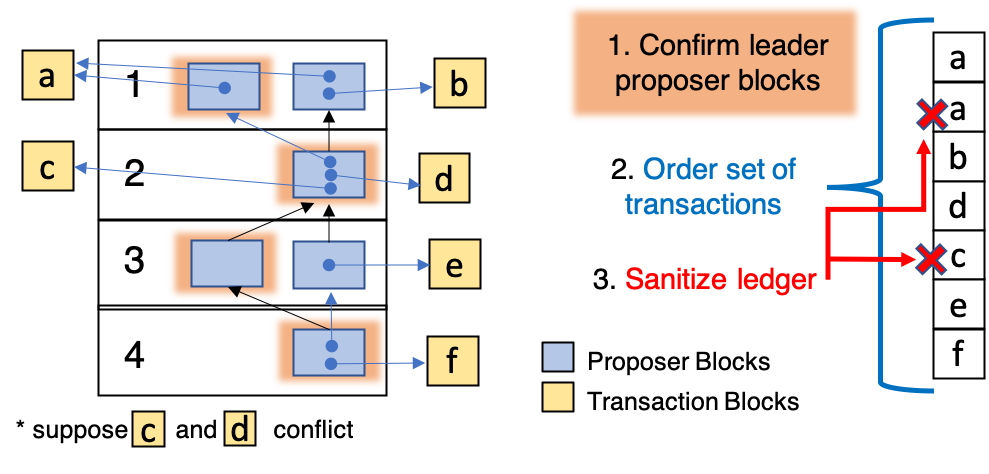
\includegraphics[width=\linewidth]{figures/ledger_generation.png}
   \vspace{-5mm}
    \caption{\small Ledger formation has three parts:  
   (1)  confirming a leader  sequence of proposer blocks;
   (2)  creating a list  of transactions;
   and (3) sanitizing the transaction list for conflicts. 
   In this figure, each transaction  block has only one transaction; suppose transactions  (c) and (d) are inconsistent (e.g., a double spend).
   A proposer block's black reference link denotes a parent link. 
    Blue links denote reference links; a proposer block can include reference links to transaction blocks as well as proposer blocks.}
   %   \gw{A typo: unrefererred $\to$ unreferred? Do we need to use the word unrefererred? Referred blocks are okay in links.}
%   Each shade of grey corresponds to an epoch. In Step 1 (line:\ref{code:txbksOrdering}), all the transaction blocks are incorporated, and in Step 2 (line:\ref{code:sanitizeLedger}), they are combined to build the ledger.
   \label{fig:leader_ledger}
    \vspace{-5mm}

 \end{figure}


\section{Ledger Formation}
\label{sec:confirmation}
% Unlike many blockchain designs, Prism allows transactions to be confirmed before they are ordered. 
% This is possible because confirmation is often an easier task than ordering. 
% For example, consider the following two transactions: a) Alice pays Bob 10\$, and b) Carol pays Drake 10\$. Both these transactions can be individually confirmed without deciding which transaction occurred first.
% The decision to separate transaction confirmation from ordering helps Prism achieve low latency. 
% However, as a result, conflicting or duplicate transactions can become part of the blockchain; these conflicts must be eliminated during transaction ordering (i.e., during ledger formation). 
% % It handles such conflicts by separating the process of confirming blocks and that of generating a ledger from the set of confirmed blocks. 
% % Without it, blockchains must maintain a single, self-consistent sequence of blocks; this causes simultaneously-mined blocks to be wasted, while slowing down the generation of the ledger. 
% % We separately discuss the two procedures of block confirmation and ledger formation. 

% \paragraph{Transaction confirmation}
Prism achieves high throughput in part by mining multiple transaction blocks simultaneously and allowing all of them to contribute to the final ledger. 
A key consequence is that blocks mined concurrently may contain redundant or conflicting transactions.
If Prism were to discard blocks that contain inconsistent transactions, it would needlessly reduce throughput by not confirming the transactions that \emph{are} consistent.
% This would also slow down transaction confirmation, because it means 
To prevent this, Prism separates the process of confirming blocks and forming a ledger. 
This is a key difference between Prism and many other blockchain protocols.
% Since the same transaction can appear in multiple Prism transaction blocks \ma{we need to give more context about why this is a problem. it's all about having a large number of transaction blocks in flight at the same time, so it's fundamentally impossible for a miner to know that a transaction it is mining has not already been included in some other transaction block by another miner}, transaction confirmation is not necessarily the same thing as transaction block confirmation. 
The formation of a ledger in Prism  occurs in three steps, as shown in Figure \ref{fig:leader_ledger}. 

\noindent{\bf (1) Proposer block confirmation.}
First, we must confirm a contiguous sequence of leader proposer blocks at each level.  
    Recall that the proposer block with the most votes on level $\ell$ is defined as the \textit{leader block} at level $\ell$, and the sequence of leader blocks for each level of the proposer tree is defined as the {\em leader sequence}. 
Once we can guarantee that this leader sequence is permanent for all levels up to some level $\ell$ with probability at least $1-\epsilon$, where $\epsilon$ is the target reversal probability, we can confirm a leader block sequence. This process is described in more detail below.

\noindent{\textbf{(2) Transaction  ordering.}}
    Given a proposer block leader sequence, we iterate over the sequence and list the referred transaction blocks in the  order they are referred. 
    We use $L_i$ to denote the leader at level $i$. 
    In Figure \ref{fig:leader_ledger}, we  start  with the leader at level 1 $L_1$, the left proposer block.
    $L_1$ refers to only one transaction  block containing transaction $a$, so our ledger starts with $a$.
    Next, we consider $L_2$. It starts by referring to its parent, the right proposer block at level 1.
    Since that proposer block has not yet been included in the ledger, we include its referred transactions---namely, $a$ and $b$. 
    $L_2$ then adds $L_1$, followed by transaction blocks containing $d$ and $c$, in that order.
    Since $L_1$ was already added to our ledger, we ignore it, but add $d$ and $c$.
    This process continues until we reach the end of our leader sequence.

\noindent{\textbf{(3) Ledger sanitization.}} In the previous step, we may have added redundant or conflicting transactions. 
    Hence, we now execute the transaction list in the previously-specified order. Any duplicate or invalid transactions are discarded. 
    In Figure~\ref{fig:leader_ledger}, we discard the second instance of $a$ (since it's a duplicate), and we discard $c$ (since it conflicts with $d$).

\if 0
\begin{enumerate}
    \item  \textbf{Proposer block confirmation.} First, we must confirm a contiguous sequence of leader proposer blocks at each level.  
    Specifically, the proposer block with the most votes on level $\ell$ is defined as the \textit{leader block} at level $\ell$. 
% This phenomenon is at the core of \schemenosp's security.
The sequence of leader blocks for each level of the proposer blocktree is defined as the {\em leader sequence}. 
Once we can guarantee that this leader sequence is permanent for all levels up to some level $\ell$ with probability at least $1-\epsilon$, we can confirm a leader block sequence. This process is described in more detail below.
    \item \textbf{Transaction  ordering.} 
    Given a proposer block leader sequence, we iterate over the sequence and list the referred transaction blocks in the  order they are referred. 
    We use $L_i$ to denote the leader at level $i$. 
    In Figure \ref{fig:leader_ledger}, we  start  with the leader at level 1 $L_1$, the left proposer block.
    $L_1$ refers to only one transaction  block containing transaction $a$, so our ledger starts with $a$.
    Next, we consider $L_2$. It starts by referring to its parent, the right proposer block at level 1.
    Since that proposer block has not yet been included in the ledger, we include its referred transactions---namely, $a$ and $b$. 
    $L_2$ then adds $L_1$, followed by transaction blocks containing $d$ and $c$, in that order.
    Since $L_1$ was already added to our ledger, we ignore it, but add $d$ and $c$.
    This process continues until we reach the end of our leader sequence.
    \item \textbf{Ledger sanitization.} In the previous step, we may have added redundant or conflicting transactions. 
    Hence, we now execute the transaction list in the previously-specified order. Any duplicate or invalid transactions are discarded. 
    In Figure \ref{fig:leader_ledger}, we discard the second instance of $a$ (since it's a duplicate), and we discard $c$ (since it conflicts with $d$).
\end{enumerate}

\fi
   
%   (3) Iterate over the transactions ledger and \emph{sanitize} it by  removing all  transactions  that conflict with a prior transaction.

% Ultimately, transaction confirmation hinges on confirmation of the proposer blocks that refer to transaction block(s) containing the transaction.
% A transaction block is confirmed once a proposer block pointing to the transaction block is confirmed.
% We thus start by explaining the confirmation of proposer blocks, then explain how this leads to transaction confirmation.


% Specifically, the proposer block with the most votes on level $\ell$ is defined as the \textit{leader block} at level $\ell$. 
% % This phenomenon is at the core of \schemenosp's security.
% The sequence of leader blocks for each level of the proposer blocktree is defined as the {\em leader sequence}. 
% Once we can confirm a contiguous leader sequence, e.g. at levels $1,\ldots, \ell$ with our desired reliability $1-\epsilon$, we can confirm an ordered ledger of transactions. 
% This ledger is formed by iterating over the sequence, and for each leader block, looping over all the transaction blocks referenced within. 
% The list of transactions from each transaction block is added sequentially to the ledger; each transaction's validity is checked for validity (e.g., double spends) and duplicate entries (since the same transaction can be added to multiple transaction blocks). 
% This process is illustrated in Figure \ref{fig:leader_ledger}. \ma{I don't really like Fig. 6. It would be better to create an example which actually shows duplicate transactions and double spends after the ordering step, and than shows the sanitized ledger. BTW, the step of going from ordered transaction blocks to order transactions doesn't seem that important (it's pretty obvious). But the most important point is that you have to do sanitization, and this has to be done after transactions are ordered. }


%\paragraph{Proposer block confirmation.} 
\smallskip
The key to the above confirmation process is leader proposer block confirmation (step 1).
The leader block at a given level $\ell$ can initially fluctuate when the voter trees start voting on level $\ell$. 
However, as the voter trees grow, votes on level $\ell$ are embedded deeper into their respective voter trees, which (probabilistically) prevents the votes from being reverted.
% A leader proposer block at a given level $\ell$ is confirmed based on the votes of the voter trees. 
Hence, we can confirm the leader block when: (1) a plurality of voter trees have voted for it, and (2) that plurality is guaranteed not to change with probability at least $1-\epsilon$, where $\epsilon$ is a user-selected target reversal probability.

%Because there are many voter trees, each individual voter tree needs  only a weak confirmation guarantee to still give a strong confirmation guarantee to the aggregate majority vote. 
% \gw{Do we need to define what is weakly confirm?}

Our confirmation procedure calculates this probability by computing a $(1-\epsilon)$-confidence interval over the number of votes on each leader block, as well as a hypothetical ``private'' block that has not yet been released by a hypothetical adversary that controls a fraction $\beta$ of the hash power. 
Once the leader block's confidence interval is strictly larger than any of the other candidates' confidence intervals, we can be sure (with probability at least $1-\epsilon$) that the current leader will remain the leader for all time, so we confirm that proposer block. 
The details of this confidence interval calculation are included in Appendix~\ref{apx:confirmation}.

\section{Spam Mitigation}
\label{sec:spamming-design}

In Prism, miners do not validate transactions before including them in blocks.
This introduces the possibility of spamming, where an adversary could generate a large number of conflicting transactions and send them to different nodes across the network.  
The nodes would then mine all of these transactions into blocks, causing miners and validators to waste storage  and computational  resources.\footnote{While a discussion of incentives is beyond the scope of this paper, it is important to note that fees alone cannot prevent such spamming. Assuming nodes only pay for transactions that make it to into the ledger, the adversary would not be charged for conflicting transactions that get removed during sanitization.}
%spam/duplicate transactions
% There are a few practical mechanisms for circumventing this. 
Notice that protocols like the longest chain are not susceptible to this attack because transactions are validated prior to block creation. 
We propose a simple mechanism to mitigate spamming. Miners validate transactions with respect to their latest ledger state and other unconfirmed transactions, giving the adversary only a small window of network delay to spam the system. 
This then allows miners to mitigate spamming attacks by adding a random timing jitter prior to mining transactions, thus increasing the chance that a miner can detect that a conflicting transaction is already present in a transaction block, in  which case it will choose to not include that transaction.
We evaluate the effectiveness of this method in \S\ref{sec:spamming-eval}.

% \smallskip


%We believe such practical countermeasures will be important in  practical settings.
%mitigations:  jitter,  mempool optimization, sortition? 

%\ma{more generally, i think we need to expand this section to explain the important parts of the design in more detail. I don't think the long pseudocode blocks are that helpful. no one will read them, and they don't distinguish the important stuff from the mundane. let's remove the pseudocode to make room to expand on things like: (1) more formal description of block contents (a diagram might help); (2) what exactly is the proof of work puzzle in prism; (3) how does sortition work; (4) how do you get the final block that is sent over the network; (5) how do we get a ledger from all these blocks; (6) how does transaction confirmation work; how and why is it different from bitcoin. there might be other stuff worth mentioning, but we should ideally describe at least each of these points at a decent level of detail} 




% Consider a proposer block sequence from levels $1$ to $\ell$, $\{p_1,\cdots,p_{\ell}\}$, represented by blue blocks in Fig. \ref{fig:leader_ledger}(a).
% Let $L_{p_i}$, represented by green blocks in the grey shaded area in Fig. \ref{fig:leader_ledger}(a), be an ordered list of all the transaction blocks directly or indirectly referred by block $p_i$. 
% Let $\{L_{p_1}, \cdots, L_{p_{\ell}}\}$ be the \textit{transaction block list} of sequence $\{p_1,\cdots,p_{\ell}\}$ as shown in Fig. \ref{fig:leader_ledger}(b). 
% We consider this transaction block list confirmed once each proposer block in the underlying sequence is confirmed. 
% Our proposer block confirmation policy is a simplified version of the policy from \cite{prism}. 
% To confirm a proposer block as leader with reliability parameter $\epsilon$, we consider the votes from all $m$ voter trees. 
% Each voter tree has some maximum probability of ending up with a vote against the block at level $1\leq i \leq \ell$.
% Once we


% While confirming a leader block can take time, 
% we quickly narrow down a set of proposer blocks, defined as the \textit{proposer set}, which is guaranteed probabilistically to contain the eventual leader block for that level. 
% The proposer set is defined as in \todo{XXX--HOW MUCH DETAIL DO WE WANT TO GO INTO? }
% % This procedure first gets all the votes from the voter trees and then gets the proposer set for each 
% % level from the genesis to the last level for which the proposer set can be realized (lines:\ref{code:getvotes_start}-\ref{code:appendPrpList}). 
% Upon  defining a proposer set for each realizable level, Prism takes an outer product of all the proposer sets to  enumerate the set of all possible proposer block leader sequences (line:\ref{code:outerproduct}). 
% Note that by design, one of these sequence will eventually be the leader block sequence.
% It then builds a ledger for each of these proposer block sequences and confirms the given transaction if it is present in \textit{all} of these ledgers (lines:\ref{code:ledgers_for_start}-\ref{code:fastConfirmTx}). 



% \textit{Confirmation and Ordering:} A set of transactions can often be individually confirmed before being ordered among themselves. 
% For this reason, confirming transactions is easier than ordering the transactions.
% For example, consider the following two transactions a) Alice pays Bob 10\$, and b) Carol pays Drake 10\$. Both these transactions can be individually confirmed without deciding which transaction occurred first.
% In Bitcoin, transactions are simultaneously confirmed and ordered; 
% however, in Prism, transactions can be confirmed before being ordered.
% The procedure \textsc{IsTxConfirmed()} in Algorithm \ref{alg:prism_con} defines the transaction confirmation rule $g$ and the procedure \textsc{GetOrderedConfirmedTxs()} defines the rule for ordering the confirmed transactions. Both these procedures use \textsc{BuildLedger()} which is described next.



% \paragraph{Transaction Ordering}
% Once a sequence of leader blocks is confirmed, the ledger is formed by iterating over the sequence, and for each leader block, looping over all the transaction blocks referenced within. 
% The list of transactions from each transaction block is added sequentially to the ledger; each transaction's validity is checked for validity (e.g., double spends) and duplicate entries (since the same transaction can be added to multiple transaction blocks). 
% This process is illustrated in Figure \ref{fig:leader_ledger}(c). 




%\ma{let's move discussion of spamming to the discussion section}

\chapter{Implementation}
\label{sec:implementation}

We have implemented a \prism client in about 10,000 lines of Rust code and can be found at~\cite{prismcode}. We describe the architecture of our implementation and highlight several design decisions that are key to its high performance.

\label{sec:implementation-architecture}

\section{Architecture}
% \vb{Similar to Bitcoin, a \textit{coin} is the fundamental entity of the currency in Prism. A coin is a $256$ length binary string which has a value and an owner. A \textit{transaction} `spends' a set of input coins and produces a new set of output coins such that the sum of the value of the input coins is equal to the sum of the value of the output coins. The output coins potentially have different owners from the input coins and this is the way users exchange money in the system.
% The \textit{history} (ledger) is defined as the ordered list of transactions and for a given history, \textit{UTXO} set is defined as the set of unspent output coins of all the transactions in the history. A transaction is valid w.r.t to a ledger iff it's input coins are in the UTXO set. Our implementation uses multi- input-multi-output transactions similar to pay-to-public-key (P2PK) in Bitcoin and Algorand~\cite{algorand, algorandcode}. We use Ed25519~\cite{ed25519} for digital signatures and SHA-256~\cite{sha256} as the hashing algorithm.}


Our implementation is based on the \textit{unspent transaction output (UTXO)} model, similar to that used by \bitcoin. UTXOs are generated by transactions. A transaction takes a list of UTXOs (\textit{inputs}) and defines a list of new UTXOs (\textit{outputs}). Each UTXO is only allowed to be spent once, and the {\em state} of the ledger, i.e., the state that results from applying the transactions that have been confirmed up to that point in the ledger, can be represented as a set of UTXOs. Our implementation features a simplified version of Bitcoin's scripting language, processing only pay-to-public-key (P2PK) transactions, similar to that implemented in Algorand~\cite{algorand, algorandcode}. We use Ed25519~\cite{ed25519} for cryptographic signatures and SHA-256~\cite{sha256} as the hashing algorithm.

% \gf{Are the previous two paragraphs supposed to be alternatives for each other? The first one doesn't mention scripting language at all, and the second one barely does. Perhaps we should change the subsection title.}\vb{Yes they are alternate of each other. I merged the two subsections into one}

%In such a system, each UTXO is associated with an owner, defined when the transaction is created, and identified by the hash of an Ed25519~\cite{ed25519} public key. To spend an UTXO, the owner must sign the transaction using the corresponding private key. In our implementation, we use Ed25519~\cite{ed25519} as the cryptographic signature scheme, and SHA-256~\cite{sha256} as the hashing algorithm. \ma{replace passive verbs with active verbs as much as possible} 

%We implement our client based on this transaction model.

\begin{figure}
    \centering
    \resizebox{0.6\textwidth}{!}{\tikzstyle{ledger} = [draw, fill=blue!20, rectangle, 
    minimum height=4em, minimum width=6em, text centered, text width=5em]
\tikzstyle{blockchain} = [draw, fill=red!20, rectangle, minimum height=4em, minimum width=6em, text centered, text width=5em]
\tikzstyle{miner} = [draw, fill=green!20, rectangle, minimum height=4em, minimum width=6em, text centered, text width=5em]

\tikzstyle{database} = [draw, fill=yellow!20, rectangle, rounded corners, text width=5em, minimum height=3em, minimum width=6em, text centered]


% The block diagram code is probably more verbose than necessary
\begin{tikzpicture}[auto, node distance=2.8cm,>=latex']
    \node [database] (blockchaindb) {Block Structure Database};
    \node [blockchain, above=0.5cm of blockchaindb] (blockchain) {Block Structure Manager};
    \node [ledger, left of=blockchaindb] (ledger) {Ledger Manager};
    \node [miner, right of=blockchaindb] (miner) {Miner};
    \node [database, left of=ledger] (utxodb) {UTXO Database};
    \node [database, right of=blockchain] (mempool) {Memory Pool};
    \node [database, left of=blockchain] (blockdb) {Block Database};
    \node [above=0.5cm of blockchain] (peers) {Peers};
    \node [right of=peers] (newtx) {New Transactions};
    \draw [<->] (blockchaindb) -- node[name=a] {} (blockchain);
    \draw [->] (blockchaindb) -- node[name=b] {} (miner);
    \draw [<->] (blockchaindb) -- node[name=c] {} (ledger);
    \draw [<-] (blockchain) -- node[name=d] {} (miner);
    \draw [<->] (miner) -- node[name=e]{} (mempool);
    \draw [->] (blockchain) -- node[name=f]{} (mempool);
    \draw [<->] (blockchain) -- node[name=g]{} (blockdb);
    \draw [<->] (ledger) -- node[name=h]{} (utxodb);
    \draw [<-] (ledger) -- node[name=i]{} (blockdb);
    \draw [<->] (peers) -- node[name=j]{} (blockchain);
    \draw [->] (newtx) -- node[name=k]{} (mempool);


\end{tikzpicture}}
    %\tikzstyle{ledger} = [draw, fill=blue!20, rectangle, 
    minimum height=4em, minimum width=6em, text centered, text width=5em]
\tikzstyle{blockchain} = [draw, fill=red!20, rectangle, minimum height=4em, minimum width=6em, text centered, text width=5em]
\tikzstyle{miner} = [draw, fill=green!20, rectangle, minimum height=4em, minimum width=6em, text centered, text width=5em]

\tikzstyle{database} = [draw, fill=yellow!20, rectangle, rounded corners, text width=5em, minimum height=3em, minimum width=6em, text centered]


% The block diagram code is probably more verbose than necessary
\begin{tikzpicture}[auto, node distance=2.8cm,>=latex']
    \node [database] (blockchaindb) {Block Structure Database};
    \node [blockchain, above=0.5cm of blockchaindb] (blockchain) {Block Structure Manager};
    \node [ledger, left of=blockchaindb] (ledger) {Ledger Manager};
    \node [miner, right of=blockchaindb] (miner) {Miner};
    \node [database, left of=ledger] (utxodb) {UTXO Database};
    \node [database, right of=blockchain] (mempool) {Memory Pool};
    \node [database, left of=blockchain] (blockdb) {Block Database};
    \node [above=0.5cm of blockchain] (peers) {Peers};
    \node [right of=peers] (newtx) {New Transactions};
    \draw [<->] (blockchaindb) -- node[name=a] {} (blockchain);
    \draw [->] (blockchaindb) -- node[name=b] {} (miner);
    \draw [<->] (blockchaindb) -- node[name=c] {} (ledger);
    \draw [<-] (blockchain) -- node[name=d] {} (miner);
    \draw [<->] (miner) -- node[name=e]{} (mempool);
    \draw [->] (blockchain) -- node[name=f]{} (mempool);
    \draw [<->] (blockchain) -- node[name=g]{} (blockdb);
    \draw [<->] (ledger) -- node[name=h]{} (utxodb);
    \draw [<-] (ledger) -- node[name=i]{} (blockdb);
    \draw [<->] (peers) -- node[name=j]{} (blockchain);
    \draw [->] (newtx) -- node[name=k]{} (mempool);


\end{tikzpicture}
    \caption{\small Architecture of our \prism client implementation.}
    \label{fig:system-architecture}
\end{figure}

The system architecture is illustrated in Figure~\ref{fig:system-architecture}. Functionally it can be divided into the following three modules:

\begin{enumerate}
    \item \textit{Block Structure Manager}, which maintains the clients' view of the blockchain, and communicates with peers to exchange new blocks.
    \item \textit{Ledger Manager}, which updates the ledger based on the latest blockchain state, executes transactions, and maintains the UTXO set.
    \item \textit{Miner}, which assembles new blocks.
\end{enumerate}
%\end{CompactEnumerate}

\noindent % follow the previous paragraph
The ultimate goal of the \prism client is to maintain up-to-date information of the blockchain and the ledger. To this end, it maintains the following four data structures:

\begin{enumerate}
    \item \textit{Block Structure Database}, residing in persistent storage, stores the graph structure of the blockchain (i.e., the voter blocktrees, proposer blocktree, and transactions blocks referenced) as well as the latest confirmed order of proposer and transaction blocks.
    \item \textit{Block Database}, residing in persistent storage, stores every block a client has learned about so far. 
    \item \textit{UTXO Database}, residing in persistent storage, stores the list of all UTXOs, as well as their value and owner.
    \item \textit{Memory Pool}, residing in memory, stores the set of transactions that have not been mined in any block.
\end{enumerate}

%For the rest of this subsection, we describe these modules and data structures, and how they interact with each other. 
%We will discuss some  highlights in detail in the next subsection.


At the core of the \textbf{Block Structure Manager} are an \textit{event loop} which sends and receives network messages to/from peers, and a \textit{worker thread pool} which handles those messages. When a new block arrives, the worker thread first checks its proof of work and sortition, according to the rules specified in \S\ref{sec:mining}, and stores the new block in the Block Database.
\footnote{Checking proof of work at the earliest opportunity reduces the risk of DDoS attacks.} 
It then proceeds to relay the block to peers that have not received it. Next, the worker thread checks whether all blocks referred to by the new block, e.g. its parent, are already present in the database. If not, it buffers the block in an in-memory data structure and defers further processing until all the block's references have been received. Once a block's references have all arrived, the worker performs further validation (e.g., verifying transaction signatures), and finally, the new block is inserted into the Block Structure Database. If the block is a transaction block, the Block Structure Manager also checks the Memory Pool against the transactions included in this new block, and removes any duplicates or conflicting ones. 

\if 0
%\smallskip
At the core of the \textbf{Block Structure Manager} are an \textit{event loop} which sends and receives network messages to/from peers, and a \textit{worker thread pool} which handles those messages. In our implementation, network messages are prefixed by their length and transported over TCP. As soon as a message is received by the event loop, it is passed on to an idle worker thread, or put into a queue if none is available. There are three types of messages: \texttt{NewBlockHashes}, which advertises the hashes of blocks that a node has just mined or received from its peers. \texttt{GetBlocks}, which asks for blocks by their hashes. And \texttt{Blocks}, which contains actual blocks. 

When a new block arrives in a \texttt{Blocks} message, the worker thread first checks its proof of work and sortition, according to the rules specified in \S\ref{sec:mining}, and stores the new block in the Block Database.\footnote{Checking proof of work at the earliest opportunity reduces the risk of DDoS attacks, because an attacker would have to solve the proof-of-work puzzle to trigger potentially costly processing at other nodes.} It then proceeds to relay the block to neighbors that have not received it, following the standard procedure implemented in \bitcoin. It broadcasts a \texttt{NewBlockHashes} message to all peers to advertise this new block. Every peer that does not have this block responds with a \texttt{GetBlocks} message to request it. 

%Advertising the new block before further processing it allows us to minimize the time for a block to propagate through the network. 
Next, the worker thread checks whether all blocks referred by the new block, e.g. its parent, are already present in the databases. If not, it buffers the block in an in-memory data structure and defers further processing until all the block's references have been received. Once a block's references have all arrived, the worker performs further validation (e.g., verifying transaction signatures), and finally, the new block is inserted into the Block Structure Database. If the block is a transaction block, the Block Structure Manager also checks the Memory Pool against the transactions included in this new block, and removes any duplicates or conflicting ones. \ma{Trim the description of the block structure managerin one paragraph. We don't need the details of the messages. The important parts seem to be: event loop + workers, it relays blocks to peers similar to bitcoin after checking proof of work and sortition, it defers processing blocks if their parents are not present in db} 

\fi 

The \textbf{Ledger Manager} is a two-stage pipeline and runs asynchronously with respect to the Block Structure Manager. Its first stage, the \textit{transaction sequencer}, runs in a loop to continuously poll the Block Structure Database and try to confirm new transactions. It starts by updating the list of votes cast on each proposer block. To avoid doing wasteful work, it caches the vote counts and the tips of the voter chains, and on each invocation, it only scans through the new voter blocks. Then, it tries to confirm a leader for each level in the proposer block tree as new votes are cast, according to the rules specified in \S\ref{sec:confirmation}. In the case where a leader is selected, it queries the Block Database to retrieve the transaction blocks confirmed by the new leader, and assembles a list of confirmed transactions. The list is passed on to the second stage of the pipeline, the \textit{ledger sanitizer}. This stage maintains a pool of worker threads that executes the confirmed transactions in parallel. Specifically, a worker thread queries the UTXO Database to confirm that all inputs of the transaction are present; their owners match the signatures of the transaction;
%~\footnote{A transaction includes both the signature and the public key of the UTXO owner. Block Structure Manager has already verified the signature against the public key. Here we check that the public key matches the owner as recorded in the UTXO Database.} 
and the total value of the inputs is no less than that of the outputs. If execution succeeds, the outputs of the transaction are inserted into the UTXO Database, and the inputs are removed.

The \textbf{Miner} module assembles new blocks according to the mining procedure described in \S\ref{sec:mining}. It is implemented as a busy-spinning loop. At the start of each round, it polls the Block Structure Database and the Memory Pool to update the block it is mining. It also implements the spam mitigation mechanism described in \S\ref{sec:spamming-design}.
Like other academic implementations of PoW systems \cite{ohie,conflux}, our miner does not actually compute hashes for the proof of work, and instead simulates mining by waiting for an exponentially-distributed random delay. Solving the PoW puzzle in our experiments would waste energy for no reason, and in practice, PoW will happen primarily on dedicated hardware, e.g., application-specific integrated circuits (ASICs). So the cost of mining will not contribute to the computational bottlenecks of the consensus protocol. %Therefore, this simplification does not introduce unrealistic artifacts.

The three databases residing in the persistent storage are all built on RocksDB~\cite{rocksdb}, a high-performance key-value storage engine. We tuned the following RocksDB parameters to optimize its performance: replacing B-trees with hash tables as the index; adding bloom filters; adding a 512 MB LRU cache; and increasing the size of the write buffer to 32 MB to sustain temporary large writes. 

\if 0
% MA: if there is anything important here include it in the description of the DBs above in 1-2 sentences

The \textbf{Block Structure Database} stores different types of links between blocks as defined in the \prism protocol: voting from voter blocks to proposer blocks; referencing from proposer blocks to proposer or transaction blocks; and parental links to proposer blocks or voter blocks. It also stores various metadata, such as the leader proposer block of a level and the order of confirmed proposer blocks. 
% the level of a voter block or a proposer block; the chain number of a voter block;  
%Although those data can all be found in the original blocks, storing them in one database allows the client to quickly follow the reference links and update the ledger. 
The \textbf{Block Database} stores every block that a node has received in its original serialized format. This allows the Block Structure Manager to forward a block to peers without paying the cost of serialization every time it is requested. The \textbf{UTXO Database} stores the mapping between a UTXO and its value and owner. This database is heavily read and written, since executing every transaction requires multiple lookups (and deletions) of the inputs and insertions of the outputs. So we tuned the following RocksDB parameters to improve its performance: replacing B-trees with hash tables as the index; adding bloom filters; adding a 512 MB LRU cache; and increasing the size of the write buffer to sustain temporary large writes. 
%Besides those persistent databases, we have the \textbf{Memory Pool} implemented as an in-memory hash table.


\fi

\section{Performance Optimizations}

\label{sec:implementation-highlights}

The key challenge to implementing the \prism client is to handle its high throughput. The client must process blocks at a rate of hundreds of blocks per second, or a throughput of hundreds of Mbps, and confirm transactions at a high rate, exceeding 70,000 tps in our implementation. To handle the high throughput, our implementation exploits opportunities for parallelism in the protocol and carefully manages race conditions to achieve high concurrency. We now discuss several key performance optimizations. 

%, and we discuss in detail those design choices in this subsection.


\noindent\textbf{Asynchronous Ledger Updates.}
In traditional blockchains like \bitcoin, blocks are mined at a low rate and clients update the ledger each time they receive a new block.  However in \prism, blocks are mined at a very high rate and a only a small fraction of these blocks\,---\,those that change the proposer block leader sequence\,---\,lead to changes in the ledger. Therefore trying to update the ledger synchronously for each new block is wasteful and can become a CPU performance bottleneck. 

%update the ledger for new block bottlenecks the system

Fortunately, \prism does not require synchronous ledger updates to process blocks. Since \prism allows conflicting or duplicate transactions to appear in the ledger and performs sanitization later (\S\ref{sec:confirmation}), the client need not update the ledger for each new block. Therefore, in our implementation, the Ledger Manager runs asynchronously with respect to the Block Structure Manager, to periodically update the ledger. 
Most blockchain protocols (e.g.,  \bitcoin, \algorand, and \bng) require that miners validate a block against the current ledger prior to mining it, and therefore cannot benefit from asynchronous ledger updates. For example, in \bitcoin's current specification, when a miner mines a block $B$, it implicitly also certifies a ledger $L$ formed by tracing the blockchain from the genesis block to block $B$. 
A \bitcoin client must therefore verify that a block \textit{B} that it receives does not contain transactions conflicting with the ledger \textit{L}, and hence must update the ledger synchronously for each block. 
In principle, \bitcoin~could perform \emph{post hoc} sanitization like \prism; however, due to long block times relative to transaction verification, doing so would not improve performance.
%\ma{If I wanted to, couldn't I just add a sanitization step to Bitcoin as well, and then allow blocks to be processed asynchronously with ledger updates?}\vb{Yes. I am not sure if async will help Bitcoin.}
%\gf{Since processing isn't the bottleneck for Bitcoin, I don't think this would help. You would still need to generate blocks slowly to prevent forking.} \pv{The reviewers may have this thought too, so how about mentioning the hypothetical that Mohammad is raising and then address it premptively in the paper itself?} \gf{added a sentence/reworded--is that ok?}

\noindent\textbf{Parallel Transaction Execution.}
\label{sec:scoreboarding}
%The high rate of transactions asserts heavy pressure on the UTXO Database in particular, since executing every transaction requires multiple lookups and deletions for the inputs, and insertions for the outputs. 
Executing a transaction involves multiple reads and writes to the UTXO Database to (1) verify the validity of the input coins, (2) delete the input coins, and (3) insert the output coins. If handled sequentially, transaction execution can quickly become the bottleneck of the whole system. Our implementation therefore uses a pool of threads in the Ledger Manager to execute transactions in parallel.\footnote{Despite parallelism, the UTXO database is the bottleneck for the entire system (\S\ref{sec:eval-resource}).}
However, naively executing all transactions in parallel is problematic, because semantically the transactions in the ledger form an order, and must be executed strictly in this order to get to the correct final state (i.e., UTXO set). For example, suppose  transactions \textit{T} and \textit{T'} both use UTXO \textit{u} as input, and \textit{T} appears first in the ledger. In this case, \textit{T'} should fail, since it tries to reuse \textit{u} when it has already been spent by \textit{T}. However, if \textit{T} and \textit{T'} are executed in parallel, race condition could happen where the inputs of \textit{T'} are checked before \textit{T} deletes \textit{u} from the UTXO Database, allowing \textit{T'} to execute.

To solve this problem, we borrow the \textit{scoreboarding}~\cite{scoreboarding} technique long used in processor design. A CPU employing this method schedules multiple instructions to be executed out-of-order, if doing so will not cause conflicts such as writing to the same register. Transactions and CPU instructions are alike, in the sense that they both need to be executed in the correct order to produce correct results, only that transactions read and write UTXOs while CPU instructions read and write CPU registers. 
In the Ledger Manager, a batch of transactions are first passed through a controller thread before being dispatched to one of the idle workers in the thread pool for execution. The controller thread keeps track of the inputs and outputs of the transactions in the batch on the scoreboard (an in-memory hash table). Before scheduling a new transaction for execution, it checks that none of its inputs or outputs are present on the scoreboard. In this way, all worker threads are able to execute in parallel without any synchronization. 
%We expect that this design choice would have even greater repercussions for more complex scripting languages, since the cost of executing each transaction would increase. 

\noindent\textbf{Functional-Style Design Pattern.}
Our system must maintain shared state between several modules across both databases and in-memory data structures, creating potential for race conditions. Further, since this state is split between the memory and the database, concurrency primitives provided by RocksDB cannot solve the problem completely. For example, to update the ledger, the Ledger Manager needs to fetch the tips of the voter chains from the memory and the votes from the Block Structure Database, and they must be in sync. Locking both states with a global mutex is a straightforward solution; however, such coarse locks significantly hurt performance. 

\if 0
Our system maintains state in several in-memory data structures, e.g., the tips of each voter chain and the list of unreferred transaction blocks. All those data are shared between modules, causing potential race conditions. Furthermore, they are split between the memory and the databases, thus concurrency primitives provided by RocksDB cannot solve the problem completely. For example, to update the ledger, the Ledger Manager needs to fetch the voter chain tips from the memory and the votes from the Block Structure Database, and they must be in sync. Locking them together with a global mutex is a straightforward solution, however, such coarse locks are not scalable. 
\fi

We adopt a functional-style design pattern to define the interfaces for modules and data structures. Specifically, we abstract each module into a function that owns no shared state. Instead, state is passed explicitly between modules as inputs and outputs. For example, the functionality of the Ledger Manager can be abstracted as $\texttt{UpdateLedger}(V, V') \rightarrow \Delta T$, where $V$ and $V'$ are the previous and current voter chain tips, and $\Delta T$ are the transactions confirmed by votes between $V$ and $V'$. Then, we design the database schema to support such functions. For example, the Block Structure Database supports the query $\texttt{VoteDiff}(V, V') \rightarrow \Delta \text{Votes}$, where $\Delta \text{Votes}$ are the added and removed votes when the voter chains evolve from $V$ to $V'$. In this way, function $\texttt{UpdateLedger}$ can invoke $\texttt{VoteDiff}$ to update the votes and confirm new transactions with no need for explicit synchronization, because each function guarantees the correctness of its output with respect to its input. Functional-style design has broader benefits than enabling global-lock-free concurrency. One example is it facilitates bootstrapping (discussed in \S\ref{sec:conclusion}), where a client needs the ledger formed by leader blocks until a certain level. Another example is reverting to a previous version of the ledgers. Such queries are easily supported in our model by calling the above update ledger function. 


%supported by a client designed in functional style.
%%\gf{Could you add a bit  more detail about why this gets rid of the need for synchronization?} \ly{done}

\noindent\textbf{No Transaction Broadcasting.}
In most traditional blockchains, clients exchange pending transactions in their memory pools with peers. This incurs extra network usage, because each transaction will be broadcast twice: first as a pending transaction, and then again as part of a block. At the throughput in which \prism operates, such overhead becomes even more significant.

Our implementation does not broadcast pending transactions, because it is \textit{unnecessary} in \prism. 
In traditional blockchains like Bitcoin and Ethereum, the whole network mines a block every tens of seconds or even few minutes. 
% \gf{I would give some examples here, just to avoid someone getting mad because their favorite blockchain  does not produce blocks at that rate}\vb{Added.}
Since we cannot predict who will mine the next block, exchanging pending transactions is necessary, so that they get included in the next block regardless of who ends up mining it. In contrast, \prism generates hundreds of transaction blocks every second. This elevated block rate means that any individual miner is likely to mine a transaction block in time comparable to the delay associated with broadcasting a transaction to the rest of the network (i.e., seconds). Hence, unlike other blockchain protocols, there is little benefit for a \prism client to broadcast its transactions. Non-mining clients can transmit their transactions to one or more miners for redundancy; however, those miners do not need to relay those transactions to peers. 




%%%%%%%%%%%%%%%



\if 0

The key challenge to implementing the \prism client is to handle its high throughput. First, blocks come to a client at a rate of hundreds of blocks per second, or a throughput of hundreds of Mbps. The client needs to process those blocks and update its view of the blockchain in real time. Second, transactions are confirmed at a high rate, higher than 70,000 tps in our implementation, and the client needs to execute transactions and update the UTXO Database at such rate. Third, transaction blocks are mined at a high rate, meaning that at any moment there are lot of transaction blocks ``in-flight'' in the network. Our design solves those challenges by exploiting parallelism in the protocol, and we discuss in detail those design choices in this subsection.


\textbf{Asynchronous Ledger Updates.}
In traditional blockchains like \bitcoin, clients try to update the ledger every time a new block is received.
However, in \prism, ledger update is much more complex. It involves accounting votes from all voter chains ($m=1000$ in our experiments) and calculating proposer leader blocks based on those votes. Performing ledger update synchronously when new blocks are received will bottleneck the system, considering that hundreds of blocks arrive every second in \prism.



(Alternate: \vb{ In traditional blockchain like \bitcoin, block are mined at a low rate and each of these blocks changes in the ledger. However in \prism, blocks are mined at a very high rate and a only a small fraction of these blocks lead to changes in the ledger and therefore trying to synchronously update the ledger for new block bottlenecks the system})

As a result, in our \prism implementation, the Block Structure Manager and the Ledger Manager do not synchronize with each other. Instead, the Ledger Manager runs repeatedly in its own loop, and updates the ledger asynchronously. Note that this design choice is uniquely applicable to \prism, for the following two reasons. First, synchronous ledger update \textit{wastes CPU resource} in \prism. In protocols with simpler blockchain structures such as \bitcoin and \algorand, every new block confirms a new set of transactions in the ledger. In such cases, updating the ledger synchronously is beneficial for minimizing the latency between receiving a block and confirming corresponding transactions. This is not the case in \prism, where confirmation occurs based on the aggregate behavior of the proposer and all voter chains;\gw{Period . rather than semicolon;} Each new block individually is very unlikely to confirm any transaction, so checking it synchronously wastes CPU power. Second, synchronous ledger update \textit{is not required by the protocol}, as opposed to \bitcoin. In \bitcoin, when a miner mines on a certain block \textit{B}, it implicitly certifies its approval of a ledger \textit{L}, formed by tracing the blockchain from the genesis block to block \textit{B}. The network thus requires~\cite{bitcoin} any block mined on \textit{B} to not contain transactions conflicting with ledger \textit{L}. As a result, in a \bitcoin client, synchronous ledger update is mandatory. This is not the case for \prism, where conflicting and duplicate transactions could appear in the ledger, and sanitization happens at a later stage.



\subsection{Concurrent Access to Block Structure Database}

As described in Section~\ref{sec:implementation-architecture}, all three modules need to access the Block Structure Database concurrently, especially the Block Structure Manager which has a pool of worker threads processing new blocks in parallel. More specifically, each worker thread in the Block Structure Manager reads the database to perform block validation and insert new data; the Ledger Manager repeatedly queries the database and updates the ledger information stored in it; and the Miner repeatedly queries the database. Although such concurrent access is not forbidden by RocksDB, no consistency is guaranteed, either. For example, the Ledger Manager could have queried the database while a Block Structure Manager thread is updating it, getting inconsistent view of the blockchain. Usually a global lock on the Block Structure Database would have solved the problem, but it greatly limits concurrency.

As a solution, we build our own atomic operations using the \textit{merge operator} and the \textit{write batch} features of RocksDB. Merge operator allows us to define arbitrary atomic read-modify-write routines, e.g. incrementing a counter or appending to a list, needed by the Block Structure Manager when inserting new blocks. Merge operators are then grouped together into write batches, whose atomicity is guaranteed by RocksDB. As a result, every worker thread in the Block Structure Manager is able to update the Block Structure Database concurrently without global lock, allowing us to process new blocks efficiently in parallel. For the Ledger Manager and the Miner, we make use of the \textit{snapshot} feature. It allows creating read-only snapshots of the database, so that multiple queries can be made on a consistent view of the blockchain. \ma{Do we take a snapshot every time the ledger manager runs? Isn't this expensive?}



\subsubsection{Parallel Transaction Execution}
\label{sec:scoreboarding}
As described earlier, transaction execution in our UTXO based system involves checking that all its inputs are present in the UTXO Database, all owners of the inputs have signed the transaction, and the total value of the inputs is no less than that of the outputs, before inserting the outputs to the database. This involves multiple reads and writes to the UTXO Database. If handled sequentially, transaction execution can quickly become the bottleneck of the whole system. A natural answer to this problem is to parallelize transaction execution, and our final implementation does so by maintaining a pool of threads in the Ledger Manager for transaction execution. However, simply doing so is problematic, because semantically the transactions in the ledger form an order, and must be executed strictly in this order to get to the correct final state, or UTXO set in our case. Consider the following scenario as a simple counterexample: suppose both transaction \textit{T} and \textit{T'} use UTXO \textit{u} as input, and \textit{T} appears first in the ledger. Normally \textit{T'} should fail, since it tries to reuse \textit{u} when it has already been used by \textit{T}. However, if \textit{T} and \textit{T'} are executed in parallel, race condition could happen where the inputs of \textit{T'} are checked before \textit{T} deletes \textit{u} from the UTXO Database, leaving \textit{T'} executed without failing.

We solve this problem by borrowing the \textit{scoreboarding}~\cite{scoreboarding} technique long used in processor design. A CPU employing this method schedules multiple instructions to be executed out-of-order, if resource is available and doing so will not cause conflicts such as writing to the same register. Transactions and CPU instructions are alike, in the sense that they both need to be executed in the correct order to produce correct results, only that transactions ``read'' and ``write'' UTXOs while CPU instructions read and write CPU registers. In the Ledger Manager, all transactions are passed through a controller thread before dispatched to one of the idling workers in the thread pool. The controller thread book-keeps the inputs and outputs of all transactions in execution on the scoreboard (an in-memory hash table). Before scheduling a new transaction for execution, it checks that none of its inputs or outputs are present on the scoreboard. In this way, all worker threads are able to execute in parallel without any synchronization. We expect that this design choice would have even greater repercussions for more complex scripting languages, since the cost of executing each transaction would increase.  


\subsubsection{Concurrent Access to Block Structure Database}

\ly{functional design, talk about future benefits. the right we believe to implement this protocol. function style state formally - ``state-passing'', then we give benefits, finally give examples. 1. multiple shared states, lead to potential race conditions. not even solvable by database. 2. give one example (voter example). 3. how to reason able race conditions to avoice coarse locks. 4. explain how the functional design pattern makes you easier to reason about race conditions. (voter example again) 5. benefits are boarder, e.g. bootstrapping become easier.}

As described in Section~\ref{sec:implementation-architecture}, all three modules need to access the Block Structure Database concurrently, especially the Block Structure Manager which has a pool of worker threads processing new blocks in parallel. More specifically, each worker thread in the Block Structure Manager reads the database to perform block validation and insert new data; the Ledger Manager repeatedly queries the database and updates the ledger information stored in it; and the Miner repeatedly queries the database. Although such concurrent access is not forbidden by RocksDB, no consistency is guaranteed, either. For example, the Ledger Manager could have queried the database while a Block Structure Manager thread is updating it, getting inconsistent view of the blockchain. Usually a global lock on the Block Structure Database would have solved the problem, but it greatly limits concurrency.

As a solution, we build our own atomic operations using the \textit{merge operator} and the \textit{write batch} features of RocksDB. Merge operator allows us to define arbitrary atomic read-modify-write routines, e.g. incrementing a counter or appending to a list, needed by the Block Structure Manager when inserting new blocks. Merge operators are then grouped together into write batches, whose atomicity is guaranteed by RocksDB. As a result, every worker thread in the Block Structure Manager is able to update the Block Structure Database concurrently without global lock, allowing us to process new blocks efficiently in parallel. For the Ledger Manager and the Miner, we make use of the \textit{snapshot} feature. It allows creating read-only snapshots of the database, so that multiple queries can be made on a consistent view of the blockchain. \ma{Do we take a snapshot every time the ledger manager runs? Isn't this expensive?}

\subsubsection{Parallel Transaction Execution}
\label{sec:scoreboarding}
As described earlier, transaction execution in our UTXO based system involves checking that all its inputs are present in the UTXO Database, all owners of the inputs have signed the transaction, and the total value of the inputs is no less than that of the outputs, before inserting the outputs to the database. This involves multiple reads and writes to the UTXO Database. If handled sequentially, transaction execution can quickly become the bottleneck of the whole system. A natural answer to this problem is to parallelize transaction execution, and our final implementation does so by maintaining a pool of threads in the Ledger Manager for transaction execution. However, simply doing so is problematic, because semantically the transactions in the ledger form an order, and must be executed strictly in this order to get to the correct final state, or UTXO set in our case. Consider the following scenario as a simple counterexample: suppose both transaction \textit{T} and \textit{T'} use UTXO \textit{u} as input, and \textit{T} appears first in the ledger. Normally \textit{T'} should fail, since it tries to reuse \textit{u} when it has already been used by \textit{T}. However, if \textit{T} and \textit{T'} are executed in parallel, race condition could happen where the inputs of \textit{T'} are checked before \textit{T} deletes \textit{u} from the UTXO Database, leaving \textit{T'} executed without failing.

We solve this problem by borrowing the \textit{scoreboarding}~\cite{scoreboarding} technique long used in processor design. A CPU employing this method schedules multiple instructions to be executed out-of-order, if resource is available and doing so will not cause conflicts such as writing to the same register. Transactions and CPU instructions are alike, in the sense that they both need to be executed in the correct order to produce correct results, only that transactions ``read'' and ``write'' UTXOs while CPU instructions read and write CPU registers. In the Ledger Manager, all transactions are passed through a controller thread before dispatched to one of the idling workers in the thread pool. The controller thread book-keeps the inputs and outputs of all transactions in execution on the scoreboard (an in-memory hash table). Before scheduling a new transaction for execution, it checks that none of its inputs or outputs are present on the scoreboard. In this way, all worker threads are able to execute in parallel without any synchronization. We expect that this design choice would have even greater repercussions for more complex scripting languages, since the cost of executing each transaction would increase.  

\subsubsection{No Transaction Broadcasting}

In most traditional blockchains, clients exchange pending transactions in their Memory Pools with peers. Doing so incurs extra network usage, because each transaction will be broadcast twice: first in its own as a pending transaction, then second in a block. At the throughput where \prism operates, such overhead becomes even more significant.

Our implementation does not broadcast pending transactions at all, because it is \textit{unnecessary} for \prism. In traditional blockchains, the whole network mines a block every tens of seconds or even few minutes. Because we can not predict who will mine the next block, exchanging pending transactions becomes necessary, so that they get included in the next block regardless of who ends up mining it. In contrast, \prism generates hundreds of transaction blocks every second. This elevated block rate means that any individual miner is likely to mine a transaction block in time comparable to the delay associated with broadcasting a transaction to the rest of the network (i.e., seconds). Hence, unlike other blockchain protocols, there is little incentive for a \prism client to broadcast its transactions. In practice, non-mining clients can transmit their transactions to one or more miners; however, those miners do not need to relay those transactions for the same reason as before.

\vb{explain How do nodes reach consensus at such a high mining rate?}

\fi

\chapter{Evaluation}
\label{sec:eval}

Our evaluation answers the following questions:

\begin{itemize}
%\begin{itemize}[leftmargin=*]
    \item What is the performance of \prism in terms of transaction throughput and confirmation latency, and how does it compare with other protocols? (\S\ref{sec:eval-performance})
    \item How well does \prism scale to larger numbers of users? (\S\ref{sec:eval-scale})
    \item How does \prism perform with limited resource, and how efficient does it utilize resource? (\S\ref{sec:eval-resource})
    %\todo{``What's the overhead of \prism in terms of CPU and network bandwidth''}
    \item How does \prism perform when under attack? (\S\ref{sec:eval-attack})
\end{itemize}

%\smallskip

\noindent{\bf Schemes compared:} We compare \prism with \algorand, \bng, and the longest chain protocol. For \bng and the longest chain protocol, we modify and use our \prism codebase to enable a fair comparison of the protocols. For \algorand, we use the official open-source implementation~\cite{algorandcode} written in Golang. Note that this implementation is different from the one evaluated in~\cite{algorand}. Therefore, we do not expect to reproduce the results in~\cite{algorand}.

\noindent{\bf Testbed:} We deploy our \prism implementation on Amazon EC2's \texttt{c5d.4xlarge} instances with 16 CPU cores, 16 GB of RAM, 400 GB of NVMe SSD, and a 10 Gbps network interface. Each instance hosts one \prism client. By default, we use 100 instances and connect them into a random 4-regular graph topology. To emulate a wide-area network, we introduce a propagation delay of 120~ms on each link to match the typical delay between two distant cities~\cite{pingmeasurement}, and a rate limiter of 400~Mbps for ingress and egress traffic respectively on each instance. We also evaluate several other network topologies (with up 1000 instances) and per-instance bandwidth limits.

To generate workloads for those experiments, we add a transaction generator in our testbed which continuously creates transactions at an adjustable rate. In our \prism implementation, the main bottleneck is RocksDB and the I/O performance of the underlying SSD, which limits the throughput to about $80,000$ tps. 
We cap transaction generation rate to 75,000 tps to avoid hitting this bottleneck.

%\ly{The \algorand implementation can support at most $4,800$ tps according to our test on the same hardware. As shown later in this section, we are not bottlenecked by it. As a result, the comparison with \algorand is fair.}

%\smallskip
\noindent{\bf Performance tuning and security:} All protocols in the experiments have design parameters, and we tried our best to tune these parameters for performance and security. For \prism, we calculate the optimal mining rate $f$ for proposer and voter blocks to achieve the best confirmation latency, given the adversarial ratio $\beta$ and desired confirmation confidence $\epsilon$. We cap the size of transaction blocks to be 40 KB, and set the mining rate for transaction blocks such that they support $80,000$ tps. Unless otherwise stated, we turn off the spam mitigation mechanism in \prism (we evaluate its effectiveness in \S\ref{sec:eval-attack}).  To ensure security, we calculate the expected {\em forking rate} $\alpha$, i.e. fraction of blocks not on the main chain, given $f$ and the block propagation delay $\Delta$. We compare $\alpha$ against the forking rate actually measured in each experiment, to ensure that the system has met the target security level. We follow the same process for \bng and the longest chain protocol. For \algorand, we adopt the default security parameters set in its production implementation. Then we hand-tune its latency parameters $\lambda$ and $\Lambda$. Specifically, we reduce $\lambda$ and $\Lambda$ until a round times out, and use the settings that yield the best confirmation latency. For \prism, we target a confirmation confidence, $\epsilon$, in the order of $10^{-9}$. For \bng and the longest chain protocol, we target $\epsilon$ in the order of $10^{-5}$. For \algorand, the blockchain halts with a probability in the order of $10^{-9}$.

\section{Throughput and Latency}
\label{sec:eval-performance}

In this experiment, we measure the transaction throughput and confirmation latency of \prism at different adversarial ratio $\beta$, and compare that with \algorand, \bng and the longest chain protocol. For \algorand, we use its default setting of security parameters, which targets $\beta=20\%$.\footnote{The maximum possible security level for Algorand is $\beta = 33\%$, but its latency is expected to increase substantially as $\beta$ approaches 33\%~\cite{algorand}.} For \bng and the longest chain protocol, we experiment with two adversarial ratios: $\beta=20\%$ and $\beta=33\%$. In both \algorand and the longest chain protocol, there is tradeoff between throughput and confirmation latency by choosing different block sizes. We explore this tradeoff and present it in a curve. For \algorand, we try block sizes between 300 KB to 32 MB. For the longest chain protocol, we try block sizes between 1.7 KB  to  33.6 MB. The parameters used in this experiment are available in Appendix~\ref{apx:datapoints}. All four protocols are deployed on the same hardware and network topology as described above. We run each experiment for a minimum of 10 minutes and report the average transaction throughput and latency. The results are shown in Figure~\ref{fig:compare}.


\noindent{\bf Throughput:}
As shown in Fig. \ref{fig:compare}, \prism is able to maintain the same transaction throughput of around $75,000$ tps regardless of the $\beta$ chosen.
This is because \prism decouples throughput from security by using transaction blocks. In this way, \prism is able to maintain the mining rate for transaction blocks to sustain a constant throughput, while changing the mining rate for other types of blocks to achieve the desired $\beta$. \bng offers a similar decoupling by entitling the miner of the latest key block to frequently produce micro blocks containing transactions. \algorand and the longest chain protocol do not offer such decoupling, so one must increase the block size in order to achieve a higher throughput. In such case, the confirmation latency increases, as demonstrated by the tradeoff curves in Figure~\ref{fig:compare}, to accommodate for the higher block propagation delay induced by larger blocks. For the longest chain protocol, its throughput limit has been discussed in \S\ref{s:lc-thput}.
For \algorand, we observe its throughput increases marginally with block size, but does not exceed $1300$ tps.
The reason is that \algorand only commits one block every round. So at any moment, unlike \prism, \algorand only has one block propagating in the network, causing low bandwidth utilization. For \bng, we observed a peak throughput of 21,530 tps. The reason is that, unlike \prism, in \bng only a single node (the leader) commits transactions at a time. This results in the network becoming a bottleneck; once throughput exceeds about 20,000 tps, we observed that the block propagation delay increases significantly for \bng.\footnote{Note also that Bitcoin-NG is susceptible to an adaptive attack that censors the chosen leader and can reduce throughput substantially~\cite{parallel}.}


\noindent{\bf Is Consensus the Throughput Bottleneck?}
A blockchain client has two roles: (1) it participates in the consensus protocol (the \textit{Block Structure Manager} and the \textit{Miner} in our implementation); (2) it executes transactions confirmed by the consensus protocol and updates the ledger (the \textit{Ledger Manager} in our implementation). The throughput can be bottlenecked by either of these stages and therefore we ask: Is the throughput limited by the consensus protocol, or the ledger updates? To answer this question, we measure the maximal throughput when no consensus protocol is involved, i.e. we start one client of each protocol and test how fast each client can execute transactions and update the ledger. For our \prism, \bng and longest chain client, the limit is around $80,000$ tps. For \algorand, the limit is around $4,800$ tps. From Fig.~\ref{fig:compare} we see that \bitcoin, \bng, and \algorand have throughput much lower than these limits, and thus are bottlenecked by the consensus protocols. However, in case of \prism, its throughput is very close to the limit, and hence it is bottlenecked by the ledger updates.

\noindent{\bf Confirmation Latency:} The confirmation latency of \prism stays below one minute for $\beta \leq 40\%$. At $\beta = 20\%$, \prism achieves a latency of $13$ seconds, and for  similar security guarantees \algorand achieves latency of $2$ seconds. Compared to the longest chain protocol, \prism uses multiple voter chains in parallel ($1000$ chains in our experiments) to provide security instead of relying on a single chain. So \prism requires each vote to be less deep in order to provide the same security guarantee. As a result, \prism achieves a substantially lower confirmation latency. For example, for $\beta = 33\%$, the confirmation latency for \prism is 23 seconds, compared to 639 seconds at the lowest throughput point for the longest chain protocol. As we increase the block size for the longest chain protocol, its  confirmation latency increases to 1956 seconds at a throughput of 282 tps. The gap between \prism and the longest chain protocol increases for higher $\beta$. For example, for \prism the confirmation latency increases from 13 seconds to 23 seconds as $\beta$ increases from $20\%$ to $33\%$. For the longest chain protocol, the same change in $\beta$ causes the latency to increase by more than 800 seconds. \bng exhibits similar confirmation latency as the longest chain protocol for the same value of $\beta$, since it applies the same $k$-deep rule as the longest chain protocol for key blocks to confirm transactions, and key blocks must be mined slowly to avoid frequent leader changes.

%that is $10\times$ better than the longest chain protocol even at its lowest .

\section{Scalability}

\label{sec:eval-scale}
\begin{table}[ht]
	\centering
	\caption{\small Performance of \prism with different network topologies.}
	\begin{tabular}{| c || c | c c c |} 
	 \hline
	 Property & \#Nodes & 100 & 300 & 1000 \\ [0.5ex] 
	 \hline\hline
	 \multirow{4}{*}{Degree $=4$}   & Diameter & 5 & 7 & 9 \\
	                                & Throughput (tps) & $7.2\times 10^4$ & $7.4\times 10^4$ & $7.4\times 10^4$ \\
	                                & Latency (s) & 40 & 58 & 67 \\
	                                & Forking & 0.119 & 0.117 & 0.112 \\
	 \hline
	 \multirow{4}{*}{Diameter $=5$} & Degree & 4 & 6 & 8 \\
	                                & Throughput (tps) & $7.2\times 10^4$ & $7.9\times 10^4$ & $7.9\times 10^4$ \\ 
	                                & Latency (s) &40 & 44 & 37 \\
	                                & Forking & 0.119 & 0.119 & 0.127 \\
	 \hline
	\end{tabular}
	\label{table:scale}
	\end{table}

In this experiment, we evaluate \prism's ability to scale to a large number of users. For each client, we use the same network and hardware configuration as in other experiments, and target an adversarial ratio $\beta=40\%$. The results are shown in Table~\ref{table:scale}.

First, we increase the number of clients while keeping the topology a random 4-regular graph, i.e., each client always connects to four random peers. In this case, the network diameter grows as the topology becomes larger, causing the block propagation delay to increase and the confirmation latency to increase correspondingly. Note that the transaction throughput is not affected\footnote{In the results, the throughput increases as we increase the network size. This is because of an artifact in our testbed which causes slightly more transactions to be generated when there are more nodes in the network.} because in \prism the mining rate for transaction blocks is decoupled from that of the other types of blocks. Then, we explore the case where clients connect to more peers as the topology grows larger, so that the diameter of the network stays the same. As shown in the results, both confirmation latency and throughput are constant as the number of clients increases from 100 to 1000. 

In all cases, the forking rate stays stable and is under $0.13$, proving that the system is secure for $\beta=40\%$. This suggests that \prism is able to scale to a large number of users, as long as the underlying peer-to-peer network provides a reasonable block propagation delay. We also provide the distributions of block propagation delay in each topology in Appendix~\ref{apx:propagation}.

\section{Resource Utilization}
\label{sec:eval-resource}

In this experiment, we evaluate the resource utilization of our \prism implementation, and how it performs with limited network bandwidth and CPU resources. 

% resources. Generally \prism uses the following three resources: CPU, to verify cryptographic signatures, to execute transactions, and to assemble blocks. Storage, to store the ledger and blocks. Network, to receive and broadcast blocks from/to peers.




\begin{figure}
    \centering
    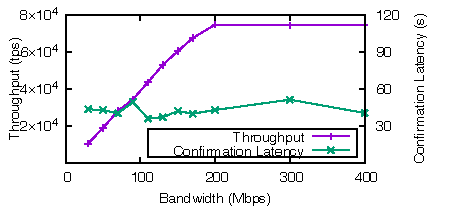
\includegraphics[width=0.75\textwidth]{figures/resource-fig-bw.pdf}
    \caption{\small Performance of \prism with different network bandwidth at each client. The in-memory size of a transaction is 168 bytes.}
    \label{fig:bw}
\end{figure}

\begin{table}[ht]
\centering
\caption{\small Network bandwidth usage breakdown of \prism measured on a 200 Mbps interface. Network Headroom is the unused bandwidth necessary for the block propagation delay to stay stable. Serialization overhead is wasted space when serializing in-memory objects for network transmission. Messaging stands for non-block messages.}
\begin{tabular}{| c | c | c || r |} 
 \hline
 \multicolumn{3}{|c||}{Usage} & $\%$Bandwidth \\ [0.5ex] 
 \hline\hline
 \multirow{5}{*}{Received} & \multirow{4}{*}{Deserialized} & Proposer Block & $0.05\%$ \\
 && Voter Block & $0.21\%$ \\
 && Transaction Block & $50.43\%$ \\ \cline{3-4}
 && Messaging &  $0.43\%$ \\ \cline{2-4} 
 & \multicolumn{2}{|c||}{Serialization Overhead} & $25.80\%$ \\ \hline
 \multicolumn{3}{|c||}{Network Headroom} & $23.08\%$ \\
 \hline
\end{tabular}

\label{table:bw-profiling}
\end{table}

\noindent{\bf Network Bandwidth:} Figure~\ref{fig:bw} shows the throughput and confirmation latency of \prism as we throttle the bandwidth at each client. Results show that the confirmation latency is stable, and the throughput scales proportionally to the available bandwidth. The throughput stops to grow when the bandwidth is higher than 200 Mbps, because the transaction generation rate is capped at 75,000 tps, which is near the bottleneck caused by RocksDB.

Table~\ref{table:bw-profiling} provides a breakdown of bandwidth usage. Our implementation is able to process transaction data at a throughput about $50\%$ of the available bandwidth. Further improvements could be made by using more efficient data serialization schemes and optimizing the underlying P2P network.

\begin{figure}
    \centering
    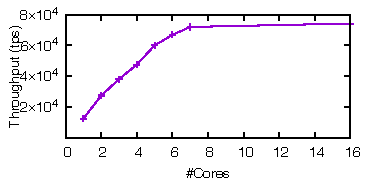
\includegraphics[width=0.65\textwidth]{figures/resource-fig-cpu.pdf}
\caption{\small Performance of \prism with different number of CPU cores at each client}
    \label{fig:cpu}
\end{figure}

\noindent{\bf CPU:} Figure~\ref{fig:cpu} shows the throughput of \prism as we change the number of CPU cores for each client. The throughput scales proportionally to the number of cores, and stops to grow after 7 cores because the transaction generation rate is capped. This shows that our implementation handles more than 10,000 tps per CPU core, and the parallelization techniques discussed in \S\ref{sec:implementation} are effective. 

Table~\ref{table:profiling} provides a breakdown of CPU usage across different components. More than half of CPU cycles are taken by RocksDB for which we only perform basic tuning. Less than $15\%$ are spent on overhead operations, such as inter-thread communication, synchronization, etc. (categorized as ``Miscellaneous'' in the table). This suggests that our implementation uses CPU resources efficiently, and further improvements could be made primarily by optimizing the database. 

While we chose mid-end AWS EC2 instances for  experiments, our results show that  \prism  does not inherently require powerful machines or waste resources.\footnote{For example, a laptop with 8 cores, 16 GB RAM, and 400 GB of NVMe-based SSD would cost under \$3,000 today and could easily run Prism.} On the contrary, its high resource efficiency and scalability that we demonstrate in this experiment makes \prism suitable for applications with different requirements. 

%This suggests that our implementation design mentioned in Section~\ref{sec:implementation-highlights} enables efficient and scalable parallelization.

\begin{table}[ht]
\centering
\caption{\small CPU usage breakdown of our \prism implementation.}
\begin{tabular}{| c | c || r |} 
 \hline
 \multicolumn{2}{|c||}{Operation} & $\%$CPU \\ [0.5ex] 
 \hline\hline
 %\multirow{5}{*}{Ledger} & RocksDB Read & $13.2\%$ \\ %\cline{2-3}
 %                        & RocksDB Write & $13.1\%$ \\ %\cline{2-3}
 \multirow{3}{*}{Ledger} & RocksDB Read/Write & $49.5\%$ \\ %\cline{2-3}
                         & (De)serialization & $3.1\%$\\ %\cline{2-3}
    %                     & Serialization & $2.0\%$\\ %\cline{2-3}
    %                     & Deserialization & $1.1\%$ \\ %\cline{2-3}
                         & Miscellaneous & $8.9\%$\\ \hline
 \multirow{5}{*}{Blockchain}    & Signature Check & $21.7\%$ \\ %\cline{2-3}
                         & (De)serialization & $3.8\%$ \\
                         & RocksDB Read/Write & $3.9\%$ \\
 %                        & Serialization & $2.0\%$\\ %\cline{2-3}
 %                        & Deserialization & $1.8\%$ \\ %\cline{2-3}
                         & Network I/O & $0.6\%$ \\ %\cline{2-3}
                         & Miscellaneous & $5.5\%$\\ \hline
% \multicolumn{2}{|c||}{RocksDB Background Jobs} & $25.0\%$ \\ \hline
  \multicolumn{2}{|c||}{Block Assembly} & $1.5\%$ \\ \hline
 \multicolumn{2}{|c||}{Transaction Generation} & $0.7\%$ \\ \hline
 \multicolumn{2}{|c||}{Miscellaneous} & $0.8\%$ \\ \hline
\end{tabular}
\label{table:profiling}
\end{table}

\section{Performance Under Active Attack}
\label{sec:eval-attack}

In the following experiments, we evaluate how \prism performs in the presence of active attacks. Specifically, we consider three  types of attacks: {\em spamming}, \textit{censorship}, and \textit{balancing} attacks. Spamming and censorship attacks aim to reduce network throughput, while balancing attacks aim to increase confirmation latency. 
%For censorship and balancing attacks, we configure a variable fraction of clients to be malicious and measure the throughput and latency of the system. 
In these experiments we configure \prism to tolerate a maximum adversarial ratio $\beta=40\%$. 

%We will demonstrate that the performance of \prism degrades gracefully under active attacks.
%\todo{cite https://eprint.iacr.org/2016/555.pdf}



\label{sec:spamming-eval}
\noindent{\bf Spamming Attack.} Recall that in a spamming attack, attackers send conflicting transactions to different nodes across the network. As described in \S\ref{sec:spamming-design}, miners can mitigate such attack by adding a random timing jitter to each transaction. In this experiment, we set up 100 miners as victims and connect them according to the same topology as in other experiments. Then for each miner we start a local process that generates a transaction every 100 ms. We synchronize those processes across the network so that each miner receives the same transaction at the same time, with a time synchronization error of several ms due to the Network Time Protocol. 
To defend against the attack, miners add a uniform random delay before including a transaction into the next transaction block. We let each attack to last for 50 seconds, and measure the fraction of spam transactions that end up in transaction blocks. 
Fig.~\ref{fig:attack-spamming} shows that adding a random jitter of at most 5 seconds can reduce the spam traffic by about 80\%. 
We point out that miners can extend this method by monitoring the reputation of clients by IP address and public key, and penalizing clients with high spam rate with longer jitter.

%\gf{Notice that the protocols we compare against (the Longest Chain protocol, Algorand, Bitcoin-NG) are not susceptible to these attacks because transactions are validated prior to block creation.}
%An adversary could generate a large number of conflicting transactions and disseminate them to different nodes across the network.  
%The 
%spam/duplicate transactions
% There are a few practical mechanisms for circumventing this. 
%To circumvent this, nodes should first validate transactions with respect to their latest ledger state and other unreferred transaction blocks, 
%\gw{I think ledger state is more proper than ledger tip.}
%giving the adversary only a small window of network delay to spam the system. % and thus significantly weakens the attack.
%Second, miners could add some timing jitter prior to mining transactions, 
%giving other miners the ability to observe if a conflicting transaction is already present in a transaction block, in  which case the miner will choose to not include that transaction. % in its block.
%We evaluate the effectiveness of this method in \S\ref{sec:spamming-eval}.

\if 0
\noindent{\bf Spamming Attack.} In Prism, miners do not validate transactions before including them in blocks. 
% This raises practical issues, namely spam. 
This introduces possible spamming attacks, where attackers send conflicting transactions to different nodes across the network. 
Nodes would then mine all of these transactions into blocks, causing miners and validators to waste storage and computational  resources.

\ly{
To circumvent this issue with Prism, we propose validating transactions with respect to their latest ledger state and other unconfirmed transactions, giving the adversary only a small window of network delay to spam the system. 
Miners can then mitigate spamming attacks by adding a random timing jitter prior to mining transactions, giving other miners the ability to observe if a conflicting transaction is already present in a transaction block, in  which case the miner will choose to not include that transaction. In this experiment, we set up 100 miners as victims and connect them according to the same topology as in other experiments. Then for each miner we start a local process that generates a transaction every 100 ms. We synchronize those processes across the network so that each miner receives the same transaction at the same time, with a time synchronization error of several ms due to the Network Time Protocol. 
To defend against the attack, miners add a uniform random delay before including a transaction into the next transaction block. We let each attack last for 50 seconds, and measure the number of transactions that end up in transaction blocks. The higher the number is, the more spam traffic the attacker has been able to create.
Fig.~\ref{fig:attack-spamming} shows that adding a random jitter of at most 5 seconds can reduce the spam traffic by about 80\%. 
We point out that miners can extend this method by monitoring the reputation of clients by IP address and public key, and penalizing clients with high spam rate with longer jitter.
} 
\gw{We also present an analysis to show that another distribution of random jitter, namely, exponential distribution is also helpful to mitigate spam attacks in Appendix~\ref{app-spam}.}

\fi

\begin{figure}
    \centering
    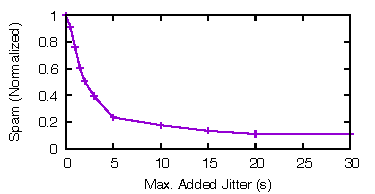
\includegraphics[width=0.65\textwidth]{figures/attack-fig-spamming.pdf}
    \caption{\small Effectiveness of random jitter in defending against spam attack. Jitters follow uniform distributions and we report the maximum jitter that we add. Spam traffic amount is normalized to the case when no jitter is added.}
    \label{fig:attack-spamming}
\end{figure}









\begin{figure}
    \centering
    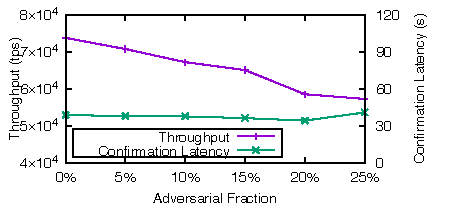
\includegraphics[width=0.75\textwidth]{figures/attack-fig-censor.pdf}
    \caption{\small Performance of \prism under  censorship attack.}
    \label{fig:attack-censor}
\end{figure}

\noindent{\bf Censorship Attack.}
In a censorship attack, malicious clients mine and broadcast empty transaction blocks and proposer blocks. Censorship attack does not threaten the security of \prism, but it reduces the system throughput because a portion of blocks are now ``useless'' since they do not contain any data. As Figure~\ref{fig:attack-censor} shows, during a censorship attack, the transaction throughput reduces proportionally to the percentage of adversarial users. Theoretically, censorship attack could also affect the confirmation latency, because it could take longer for a transaction block to be referred to if some proposer blocks are empty. However, since a proposer block is mined roughly every 10 seconds, the impact on latency is nominal. Our results shows that the confirmation latency stays stable as we increase the adversarial ratio from $0\%$ to $25\%$.


\label{sec:balancing}

\begin{figure}
    \centering
    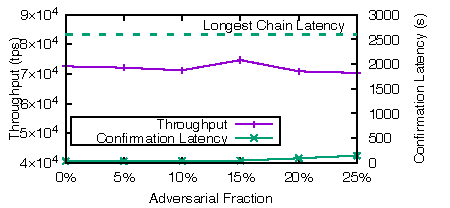
\includegraphics[width=0.75\textwidth]{figures/attack-fig-balancing.pdf}
    \caption{\small Performance of \prism under balancing attack. We also mark the confirmation latency of the longest chain protocol with the same security guarantee.}
    \label{fig:attack-balancing}
\end{figure}

\noindent{\bf Balancing Attack.}
In a balancing attack, attackers try to increase the confirmation latency of the system by waiting for the event when multiple proposer blocks appear on the same level, and then balancing the votes among them. Normally, when multiple proposer blocks appear on one level, every client votes for the proposer block with the most votes, so the system quickly converges with the vast majority of voter chains voting for one proposer block. During a balancing attack, however, the attacker votes on the proposer blocks with second most votes to slow down such convergence, causing votes to be more evenly distributed among competing proposer blocks. In this case, clients need to wait for votes to grow deeper in order to confirm a proposer leader, resulting in longer confirmation latency. Figure~\ref{fig:attack-balancing} shows that the confirmation latency grows as the active adversarial fraction increases. But even when $25\%$ clients are malicious, the confirmation latency is still more than $10\times$ better than the longest chain protocol. Meanwhile, the throughput stays stable, because such attack only targets voter blocks.


\section{conclusion}
\label{sec:conclusion}

This paper presented the implementation and evaluation of a Bitcoin-like system based on the Prism consensus protocol. Our implementation supports over 70,000 transactions per second at a confirmation latency of tens of seconds with Bitcoin-level security. Our results validate the theoretical analysis of the Prism protocol, and highlight the importance of optimizing transaction execution and the databases for high throughput.   We also demonstrated experimentally that Prism is robust to several active attacks, and showed that a simple jittering approach is effective at mitigating spamming. 

There are several avenues for future work. Our current implementation uses a UTXO-based scripting layer, and extending it to a more complex scripting layer for smart contracts is of interest.  As described in \S\ref{sec:scoreboarding}, parallelizing transaction execution (via \textit{scoreboarding}) was vital in achieving high throughput. The ability to parallelize transaction execution for smart contracts will  be  key to exploiting the high throughput provided by \prism consensus. Other extensions include methods to bootstrap new users and support light clients who only download the block headers (but not full blocks). Efficient bootstrapping is particularly important in a protocol like Prism that operates near network capacity, since expecting a new user to download and process all the old blocks is not practical. 

%An interesting direction is to store all the unspent coins in the ledger formed by leader blocks until level $\ell$ in a Merkle-Patricia tree and add the root of this tree to the proposer block(s) at level $\ell+e$ (for a large value of $e$, say $20$). Since this tree contains only unspent coins generated by valid transactions, it provides a snapshot of the state of the ledger until level $\ell$.  

\if 0
the merkle proof of the output coins of a payment with respect to to this commit proves the validity of the payment. 

 A natural question is whether we can achieve similar performance on a smart contract layer. 
 \prism's latency depends only on the block structure at the consensus layer and is independent of the scripting layer. Thus a smart contract version of Prism will also achieve low confirmation latency. 

% \smallskip
\noindent \textbf{Light clients.} 
 SPV (Simple payment verification) are short proofs~\cite{spv} to verify the validity of a given transaction (payment) for a \textit{light user} who only downloads the blocks headers in a blockchain.
In the longest chain protocol, every transaction in the block is valid so a Merkle proof of a transaction with respect to its block header proves payment validity.
However, this is not enough in \prism, where transaction blocks can potentially contain invalid transactions. We can facilitate SPV proofs in \prism by this simple modification: We store all the unspent coins in the ledger formed by leader blocks until level $\ell$ in a Merkle-Patricia tree and add the root of this tree to the proposer block(s) at level $\ell+e$ (for a large value of $e$, say $20$). Since this tree contains only unspent coins generated by valid transactions, the merkle proof of the output coins of a payment with respect to to this commit proves the validity of the payment.

% \smallskip
\noindent \textbf{Bootstrapping a new user.} 
Longest chain blockchains like Bitcoin use a small fraction of network bandwidth, so new users can simply download and process all the blocks to join the system. 
Since Prism runs near network capacity,  expecting a new user to download and process all the old blocks is not practical. 
The modification suggested in the previous paragraph can be also used to bootstrap as follows: a new user downloads all proposer and voter tree blocks (which consume less than $0.1\%$ of the capacity). Say the new user's proposer tree has confirmed leader block at level $\ell$. 
We know that this leader block stores the commit of all the unspent coins up to level $\ell-e$. 
Now the new user asks an existing user for the UTXO set for the ledger up to level $\ell-e$. The user can verify the correctness of this set by comparing it with the UTXO set commitment stored in the leader block at level $\ell$.
% \gw{"the commit of stored the leader block" contains a typo?}
This UTXO set contains all the information required from transaction blocks
% \gw{can we abbr transaction to tx?}
referred by proposer blocks until level $\ell-e$ and thus the new user can join the system by downloading full blocks starting from level $\ell-e$.



\noindent \textbf{Smart contracts.} 
 Our current implementation achieves high throughput and low latency on an UTXO based scripting layer. 
 A natural question is whether we can achieve similar performance on a smart contract layer. 
 \prism's latency depends only on the block structure at the consensus layer and is independent of the scripting layer. Thus a smart contract version of Prism will also achieve low confirmation latency. As described in \S\ref{sec:scoreboarding}, parallelizing transaction execution (via \textit{scoreboarding}) was vital in achieving high throughput. The ability to parallelize transaction execution of smart contracts will also be the key to exploit the high throughput provided by \prism consensus. 
 
\fi
\appendix
\chapter{Testbed Design}
\label{apx:testbed}

In this appendix, we provide the design details of our testbed that enables us to evaluate Prism on up to 1000 EC2 virtual machines. The testbed consists of a script written in 1000 lines of \texttt{Bash} that manages the EC2 cluster, and a tool written in 1200 lines of \texttt{Golang} that collects experimental data.

\section{Working with an EC2 Cluster}

The testbed runs on Amazon EC2's \texttt{c5d.4xlarge} instances. This type of instance has 16 vCPUs, 16 GB of RAM, 400 GB of NVMe SSD, and a 10 Gbps network interface. Before starting an experiment, our Bash script calls the API of AWS to start the required instances. We noticed that sometimes the AWS datacenter (US East, Ohio) may run out of capacity and was unable to provide the instances. The situation usually resolves within a few minutes as the datacenter auto-provisions more instances of the type, and our script is written to handle this issue.

After the instances are started, the script queries the IP addresses of the instances through AWS API and writes to the local SSH config file to enable pubkey-authenticated login. It then generates a payload for each instance, including the binary of the Prism client and the full command that starts the client. To deploy the payload, instead of sending to individual servers through \texttt{scp}, it first uploads the payload to AWS S3 and controls each VM to download the payload from S3, avoiding sending the large binary files through the internet multiple times. It then mounts the NVMe storage on each VM, and configures the network bandwidth limiter and sets up an artificial delay to mimic the real internet. Specifically, we limit the total egress and ingress bandwidth respectively. While it is straightforward to shape the egress traffic by setting up \texttt{qdisc}, Linux does not allow traffic shaping of ingress traffic directly. As a solution, we forward all ingress traffic to an \texttt{ifb} device, and set up \texttt{qdisc} on this device. Finally, we tune the TCP send and receive buffer sizes to make sure the bandwidth is fully utilized.

In addition to provisioning EC2 VMs, the Bash script also has a few features to help us debug the testbed. Specifically, we found that being able to easily profile the program using Flamegraph is very useful for performance debugging and encourages us to fine-tune the program, especially since our local development machine alone does not have the hardware resource to achieve a high transaction throughput and forbids us to reproduce performance issues locally. Also, we added a function to remotely check the correctness of the system, e.g. whether all instances reach consensus and agree on the same UTXO set. This feature allowed us to capture many obscure race conditions.

\section{Monitoring the performance}

To monitor the experiment, we wrote a tool in Golang that communicates with the HTTP API of our Prism client. It periodically queries the clients and displays the following performance metrics: generated transactions, confirmed transactions, deconfirmed transactions, local network queue length, mined blocks, local block propagation delay, received blocks, confirmation latency, and forking. It also stores the time-series data in a local round-robin database and plots the data in real-time. We found that having the ability to monitor many metrics of the system is very useful for debugging, especially when the cluster involves hundreds of VMs. For example, we discovered a performance bug due to bad usage of Mutex when we noticed unusual spikes of network queuing latency. Also, collecting time-series data in real-time allows us to display the results in a Grafana dashboard during presentations and demos.

\chapter{Confirmation Rule}
\label{apx:confirmation}

In this appendix we give the detailed calculation of the confidence intervals of the votes a proposer block receives. It is used when confirming a leader proposer block, as mentioned in \S\ref{sec:confirmation}.

Consider the scenario where there are $n$ proposer blocks at level $l$, and let $\mathcal P =\{B^P_1, B^P_2, \ldots, B^P_n\}$ denote the set of proposer blocks at level $l$. Now we want to count the number of votes each block will get with confidence $1-\epsilon$.

Suppose $B^P_i$ gets $v_i$ votes. Here a vote stands for a voter block which is on the longest chain of its voter tree and votes for $B^P_i$. 
Let $\mathcal V_i =\{B^V_{i_1}, B^V_{i_2}, \ldots, B^V_{i_{v_i}}\}$ denote the set of votes that $B^P_i$ has. For every vote $B^V_{i_j}$, let $d_{i_j}$ denote its depth, which is the number of blocks appended to voter block $B^V_{i_j}$ in the longest chain, plus one.

Now, for each vote $B^V_{i_j}$ with depth $d_{i_j}$, we want to calculate the probability $P_{i_j}$ of it being permanent. 
% \textit{not} being overtaken by a hypothetical, unreleased adversarial chain any time in the future. 
To do so, we consider a potential private double-spend attack, assuming an adversarial party is trying to overturn the voting results to elect a different proposer block $B^P_A$ as the leader block of level $l$. 
Note that $B^P_A$ could either be a block in $\mathcal P$, i.e. publicly known, or a block the adversary has privately mined but not released. 
To elect $B^P_A$ as the leader block of level $l$, the adversarial party would need to mine its own voter chains to overturn some existing votes to vote for $B^P_A$. 

We want to compute the probability of this happening.
% we need to reason about the blocks the adversary has already mined as well as those it will mine in the future. 
However, we do not know when the adversary started mining voter blocks for $B^P_A$.
% , which means we do not know how long the adversary could have been mining its private blocks. 
% However, from the visible state of the blockchain, we can estimate when $B^P_i$ was mined; assuming $B^P_A$ was mined at least as late as $B^P_i$, this gives us a bound. 
Notice that the adversary has no incentive to mine voter blocks for $B^P_A$ until $B^P_i$ has been mined and released. 
Since the honest nodes are always releasing blocks, we can use the average depth of the votes for $B^P_i$ in the public voter trees to estimate the time passed since $B^P_i$ was released, hence  bounding the expected number of votes the adversary could have accumulated on their private fork in the same amount of time. 
That is, since block inter-arrivals are exponentially distributed, the number of blocks mined since block $B^P_i$ was proposed is a Poisson random variable, with rate equal to its mean. 
This quantity can be related to the time elapsed since $B^P_i$ was released via the block mining rate.
% To do this, we estimating how deep those private voter chains are on average. 

More precisely, as an honest node, we assume the fraction of adversarial hashing power is $\beta$, and we can empirically estimate the average depth of existing public votes as $\bar{d}=\sum_{ij}{d_{i_j}}/\sum_{i}{v_i}$ and the forking rate $\alpha$~\footnote{The fraction of blocks not on the longest chain out of all blocks.} of public voter chains. 
Since there are many voter chains, these estimates converge quickly to their true means. 
Then, we calculate the estimated average depth of a \emph{private} voter chain, denoted as $\bar{d_A}$, to be
% \gf{Yes, the sentences starting with "we observe that" to the end of this para  (through the following equations) need a good bit more explanation. Minor nits: In the defn of $\bar{d}$, $v_i$ was earlier defined as the total number of votes, not the honest number  of votes,
% but $\bar{d}$ is defined as the average depth of honest votes. How are you defining an "honest vote" here? 
% Also, the sentence starting with "We observe" doesn't parse.}
% \ly{``honest'' is better defined as ``public'' here, and I have changed the definitions correspondingly. Also, I added the sentence below the next equation. Does this sound like enough explanantion?}
$$\bar{d_A} = \frac{\beta \bar{d}}{(1-\alpha)(1-\beta)}.$$
Here the $1/(1-\alpha)$ term accounts for forking in public voter chains and assumes that the malicious private voter chains do not fork. The $\beta / (1-\beta)$ term accounts for the ratio of hashing power between the honest users ($1-\beta$) and the malicious users ($\beta$).
This expected depth $\bar{d_A}$ can be used as an estimate of the rate of the Poisson random variable of the number of blocks in the adversary's  private chain. 


Since each voter chain follows the longest-chain rule, the calculation for $P_{i_j}$ is the same as in \bitcoin
$$P_{i_j} = F_{\text{Pois}}(d_{i_j};\bar{d_A}) - \sum_{k=0}^{d_{i_j}}f_{\text{Pois}}(k;\bar{d_A})\frac{\beta}{1-\beta}^{d_{i_j} + 1 - k}.$$
Here $F_{\text{Pois}}(x;\lambda)$ is the cumulative distribution function and $f_{\text{Pois}}(x;\lambda)$ is the probability mass function of Poisson distribution with rate parameter $\lambda$.
In this expression, the first term is the probability that the adversary has mined fewer than $d_{i_j}+1$ blocks, in which case it cannot currently overtake the main chain. 
The second term computes, for each possible length of the adversary's chain, the probability that the adversary overtakes the public voter chain in the future by mining faster. 

Given $P_{i_j}$, we can now calculate the confidence interval of votes on each proposer block. For proposer block $B_i^P$ and each of its votes $B^V_{i_j}$, let $\tilde V_{i_j}$ be the random variable where
$$\tilde V_{i_j} = \begin{cases}
    1, & \text{if vote } B^V_{i_j} \text{ is secure forever (permanent)} \\
    0, & \text{if vote } B^V_{i_j} \text{ will be overturned}
  \end{cases}.$$
With some abuse of notation, let $v_i$ be the random variable equal to the number of secure votes of $B^P_i$. We have
$$v_i = \sum_{j}B^V_{i_j}.$$
Note that $\tilde V_{i_j}\sim \text{Bernoulli}(P_{i_j})$. Then the lower confidence bound of votes on $B_i^P$ (denoted as $\left \lfloor v_{i} \right \rfloor$) can be obtained by calculating in $\epsilon$-quantile of random variable $v_i$.

In real-world implementations, given the complexity of such computation, its closed-form approximation may be used. We can approximate $v_i$ using a Gaussian distribution $\mathcal N(\mu_i, \sigma_i^2)$ where
$$\mu_i=\sum_j P_{i_j}.$$
$$\sigma_i^2 = \sum_j P_{i_j}(1-P_{i_j}).$$
Using the closed-form approximation of the quantile function of normal distribution, we have
$$\left \lfloor v_{i} \right \rfloor \approx \mu_i - \sigma_i \sqrt{\ln{
\frac{1}{\epsilon^2}} - \ln{\ln{\frac{1}{\epsilon^2}}} - \ln{(2\pi)}}.$$

Now, we consider the upper confidence bound of votes on $B_i^P$ (denoted as $\left \lceil v_{i} \right \rceil$). Here, we want to defend against the worst case where for each $B_i^P$, only $\left \lfloor v_{i} \right \rfloor$ votes are retained, and the adversarial party controls the remaining votes (we let $\left \lceil v_A \right \rceil$ denote the number of such votes). Recall that each voter chain can only vote for each proposer level once. For a system with $m$ voter chains, we have
$$\left \lceil v_A \right \rceil = m - \sum_{i}\left \lfloor v_{i} \right \rfloor.$$
The adversarial party will use those votes to vote for $B^P_A$. Since $B^P_A$ could be any block in $\mathcal P$, we have
$$\left \lceil v_i \right \rceil = \left \lfloor v_{i} \right \rfloor + \left \lceil v_A \right \rceil.$$
$B^P_A$ could also be a block which the adversarial party mines but has not released. In such case, the upper bound of votes on $B^P_A$ is just $\left \lceil v_A \right \rceil$. Finally, to select the leader of level $l$, we search for the block $B^P_L \in \mathcal P$ satisfying $\left \lfloor v_{L} \right \rfloor > \left \lceil v_i \right \rceil$ for every $i \neq L$ and $\left \lfloor v_{L} \right \rfloor > \left \lceil v_A \right \rceil$. In words, we select the block whose lower bound of votes is higher than the upper bound of any other known or unknown proposer block in the same level.

\chapter{Parameters Used in the Evaluation}
\label{apx:datapoints}

Here we present the parameters used in the experiment in \S\ref{sec:eval-performance} for \prism (Table~\ref{table:prism-params}, Table~\ref{table:prism-beta}), \algorand (Table~\ref{table:algorand-params}), \bng (Table~\ref{table:bng-params}), and the longest chain protocol (Table~\ref{table:lc-params}).

\begin{table}[t]
	\centering
	\caption{Parameters of \prism.}
	%\resizebox{\columnwidth}{!}{
	\begin{tabular}{ r | c } 
	 \hline
	 Parameter & Value \\ [0.5ex] 
	 \hline\hline
	 Transaction Block Size & 228 transactions \\
	 Voter Block Size & 1000 votes \\
	 Proposer Block Size & 7000 references \\
	 Voter Chains ($m$) & 1000 \\
	 Transaction Mining Rate & 350 Blocks/s \\
	 Voter Mining Rate & Table~\ref{table:prism-beta}\\
	 Proposer Mining Rate & Table~\ref{table:prism-beta}\\
	 \hline
	\end{tabular}
	%}
\label{table:prism-params}
\end{table}

\begin{table}[t]
	\centering
        \caption[Mining rate of proposer and voter blocks in Prism.]{Mining rate $f$ of proposer and voter blocks for different $\beta$ in \prism. The unit is Blocks/s.}
	%\resizebox{\columnwidth}{!}{
	\begin{tabular}{ r | c } 
	 \hline
	 $\beta$ & Mining Rate ($f$) \\ [0.5ex] 
	 \hline\hline
	 0.20 & 0.535 \\
	 0.33 & 0.185 \\
	 0.40 & 0.097 \\
	 0.42 & 0.081 \\
	 0.43 & 0.069 \\
	 0.44 & 0.054 \\
	 \hline
	\end{tabular}
	%}
\label{table:prism-beta}
\end{table}


\begin{table}[t]
	\centering
        \caption[Parameters of \algorand.]{Parameters of \algorand. Block Size: number of transactions in a block. Assembly Time: maximum time spent on assembling a block (this limit was never hit in the experiment). $\lambda$: expected time to reach consensus on block hash. $\Lambda$: expected time to reach consensus on the actual block. Detailed definition in~\cite{algorand}.}
	%\resizebox{\columnwidth}{!}{
	\begin{tabular}{ r | c | c | c } 
	 \hline
	 Block Size & Assembly Time (s) & $\lambda$ (s) & $\Lambda$ (s) \\ [0.5ex] 
	 \hline\hline
	 1287 & 0.5 & 0.6 & 1.6 \\
	 4366 & 0.8 & 1.2 & 3.0 \\
	 8733 & 1.6 & 1.9 & 6.5 \\
	 13100 & 1.6 & 1.9 & 10.0 \\
	 17294 & 1.6 & 2.0 & 13.0 \\
	 21504 & 1.9 & 2.3 & 16.0 \\
	 42334 & 3.5 & 3.9 & 38.0 \\
	 64614 & 5.0 & 5.4 & 56.0 \\
	 85513 & 7.0 & 7.4 & 73.0 \\
	 85836 & 7.0 & 7.4 & 68.0 \\
	 103004 & 8.4 & 8.8 & 84.0 \\
	 116580 & 9.5 & 9.9 & 99.0 \\
	 133766 & 11.0 & 11.4 & 110.0 \\
	 \hline
	\end{tabular}
	%}
\label{table:algorand-params}
\end{table}

\begin{table}[t]
	\centering
	\caption{Parameters of \bng.}
	\begin{tabular}{ r | c } 
	 \hline
	 Parameter & Value \\ [0.5ex] 
	 \hline\hline
	 Key Block Mining Rate & 0.10 Block/s \\
	 Micro Block Interval & 15000 $\mu\text{s}$ \\
	 Block Size & 500 transactions \\
	 \hline
	\end{tabular}
\label{table:bng-params}
\end{table}

\begin{table}[t]
	\centering
        \caption[Mining rate in the longest chain protocol.]{Mining rate $f$ for different $\beta$ and block sizes in the longest chain protocol. Here block sizes are in terms of transactions.}
	%\resizebox{\columnwidth}{!}{
	\begin{tabular}{ r | r | c } 
	 \hline
	 $\beta$ & Block Size & Mining Rate ($f$) \\ [0.5ex] 
	 \hline\hline
	 \multirow{8}{*}{0.20} & 10 & 0.404 \\
	                       & 260 & 0.262 \\
	                       & 1000 & 0.221 \\
	                       & 4000 & 0.144 \\
	                       & 10000 & 0.110 \\
	                       & 20000 & 0.079 \\
	                       & 60000 & 0.064 \\
	                       & 200000 & 0.027 \\
	 \hline
	 \multirow{4}{*}{0.33} & 10 & 0.168 \\
	                       & 260 & 0.117 \\
	                       & 1000 & 0.119 \\
	                       & 4000 & 0.065 \\
	 \hline
	\end{tabular}
	%}
\label{table:lc-params}
\end{table}





\chapter{Block Propagation Delay Distribution}
\label{apx:propagation}

 Here we present the distribution plots of the block propagation delay ($\Delta$) in topologies tested in our scalability experiment (\S\ref{sec:eval-scale}). The data are shown in Figures~\ref{fig:propagation1}, \ref{fig:propagation2}, \ref{fig:propagation3}, \ref{fig:propagation4}, \ref{fig:propagation5}. In each plot, the concrete lines mark the mean of the propagation delay of that type of blocks, and the dashed lines mark the $25\%$ and $75\%$ quantiles. Comparing Figures~\ref{fig:propagation1}, \ref{fig:propagation3}, \ref{fig:propagation5} we observe that as long as the network diameter is kept constant, the block propagation delay is barely affected by the increase of clients.


\begin{figure}[t]
   \centering
   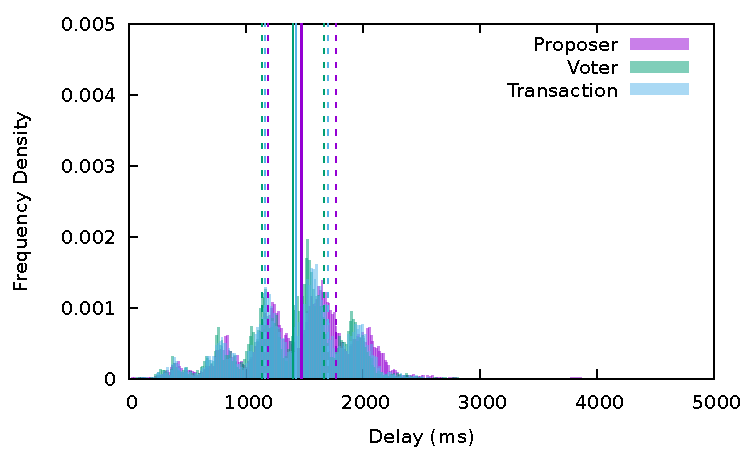
\includegraphics[width=\linewidth]{figures/delay100nodes.pdf}
   \caption{Block propagation delay. Nodes$=100$, Degree$=4$, Diameter$=5$}%\vspace{-6mm}
   \label{fig:propagation1}
 \end{figure}
 
 \begin{figure}[t]
   \centering
   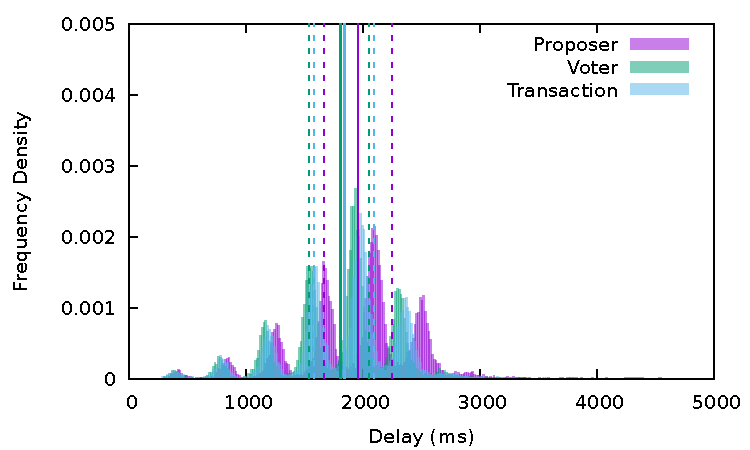
\includegraphics[width=\linewidth]{figures/delay300nodes4.pdf}
   \caption{Block propagation delay. Nodes$=300$, Degree$=4$, Diameter$=7$}%\vspace{-6mm}
   \label{fig:propagation2}
 \end{figure}
 
 \begin{figure}[t]
   \centering
   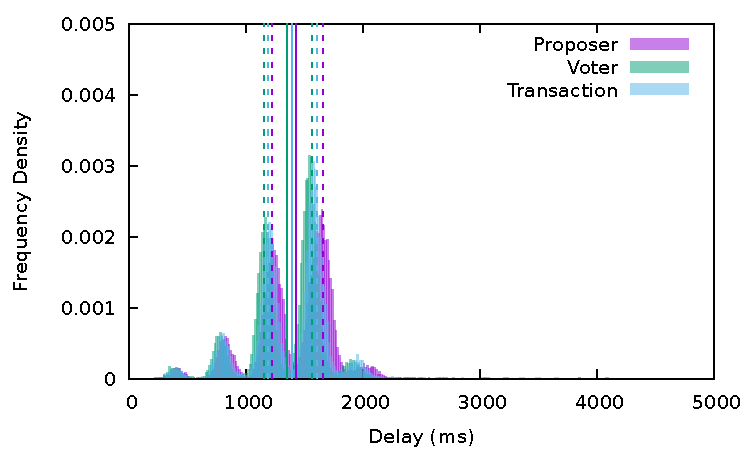
\includegraphics[width=\linewidth]{figures/delay300nodes6.pdf}
   \caption{Block propagation delay. Nodes$=300$, Degree$=6$, Diameter$=5$}%\vspace{-6mm}
   \label{fig:propagation3}
 \end{figure}
 
 \begin{figure}[t]
   \centering
   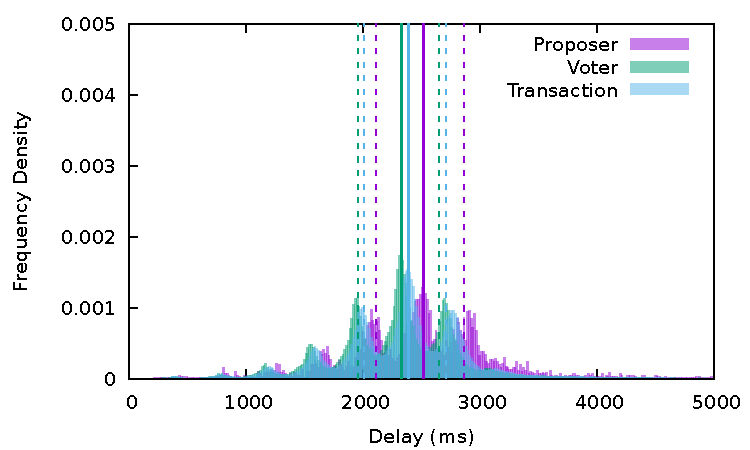
\includegraphics[width=\linewidth]{figures/delay1000nodes4.pdf}
   \caption{Block propagation delay. Nodes$=1000$, Degree$=4$, Diameter$=9$}%\vspace{-6mm}
   \label{fig:propagation4}
 \end{figure}
 
 \begin{figure}[t]
   \centering
   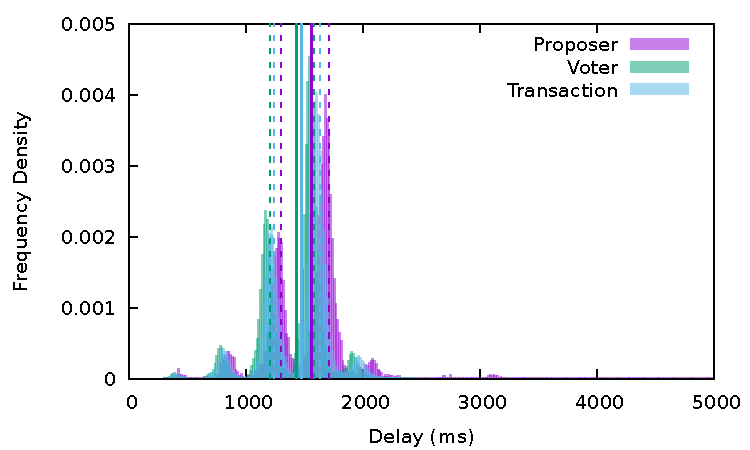
\includegraphics[width=\linewidth]{figures/delay1000nodes8.pdf}
   \caption{Block propagation delay. Nodes$=1000$, Degree$=8$, Diameter$=5$}
   \label{fig:propagation5}
 \end{figure}
 


%% This defines the bibliography file (main.bib) and the bibliography style.
%% If you want to create a bibliography file by hand, change the contents of
%% this file to a `thebibliography' environment.  For more information 
%% see section 4.3 of the LaTeX manual.
\begin{singlespace}
\bibliography{main}
\bibliographystyle{plain}
\end{singlespace}

\end{document}

